%%%%%%%%%%%%%%%%%%%%%%%%%%%%%%%%%%%%%%%%%
% The Legrand Orange Book
% LaTeX Template
% Version 2.0 (9/2/15)
%
% This template has been downloaded from:
% http://www.LaTeXTemplates.com
%
% Mathias Legrand (legrand.mathias@gmail.com) with modifications by:
% Vel (vel@latextemplates.com)
%
% License:
% CC BY-NC-SA 3.0 (http://creativecommons.org/licenses/by-nc-sa/3.0/)
%
% Compiling this template:
% This template uses biber for its bibliography and makeindex for its index.
% When you first open the template, compile it from the command line with the 
% commands below to make sure your LaTeX distribution is configured correctly:
%
% 1) pdflatex main
% 2) makeindex main.idx -s StyleInd.ist
% 3) biber main
% 4) pdflatex main x 2
%
% After this, when you wish to update the bibliography/index use the appropriate
% command above and make sure to compile with pdflatex several times 
% afterwards to propagate your changes to the document.
%
% This template also uses a number of packages which may need to be
% updated to the newest versions for the template to compile. It is strongly
% recommended you update your LaTeX distribution if you have any
% compilation errors.
%
% Important note:
% Chapter heading images should have a 2:1 width:height ratio,
% e.g. 920px width and 460px height.
%
%%%%%%%%%%%%%%%%%%%%%%%%%%%%%%%%%%%%%%%%%

%----------------------------------------------------------------------------------------
%	PACKAGES AND OTHER DOCUMENT CONFIGURATIONS
%----------------------------------------------------------------------------------------

\documentclass[11pt,fleqn,openany]{book} % Default font size and left-justified equations

%----------------------------------------------------------------------------------------

%%%%%%%%%%%%%%%%%%%%%%%%%%%%%%%%%%%%%%%%%
% The Legrand Orange Book
% Structural Definitions File
% Version 2.0 (9/2/15)
%
% Original author:
% Mathias Legrand (legrand.mathias@gmail.com) with modifications by:
% Vel (vel@latextemplates.com)
% 
% This file has been downloaded from:
% http://www.LaTeXTemplates.com
%
% License:
% CC BY-NC-SA 3.0 (http://creativecommons.org/licenses/by-nc-sa/3.0/)
%
%%%%%%%%%%%%%%%%%%%%%%%%%%%%%%%%%%%%%%%%%

%----------------------------------------------------------------------------------------
%	VARIOUS REQUIRED PACKAGES AND CONFIGURATIONS
%----------------------------------------------------------------------------------------

\usepackage[top=3cm,bottom=3cm,left=3cm,right=3cm,headsep=10pt,a4paper]{geometry} % Page margins

\usepackage{graphicx} % Required for including pictures
\graphicspath{{Pictures/}} % Specifies the directory where pictures are stored

\usepackage{lipsum} % Inserts dummy text

\usepackage{tikz} % Required for drawing custom shapes

\usepackage[english]{babel} % English language/hyphenation

\usepackage{blindtext}
%\usepackage{draftwatermark}

\usepackage{enumitem} % Customize lists
\setlist{nolistsep} % Reduce spacing between bullet points and numbered lists

\usepackage{booktabs} % Required for nicer horizontal rules in tables

\usepackage{xcolor} % Required for specifying colors by name
\definecolor{ocre}{RGB}{243,102,25} % Define the orange color used for highlighting throughout the book

\usepackage{listings}

%----------------------------------------------------------------------------------------
%	FONTS
%----------------------------------------------------------------------------------------

\usepackage{avant} % Use the Avantgarde font for headings
%\usepackage{times} % Use the Times font for headings
\usepackage{mathptmx} % Use the Adobe Times Roman as the default text font together with math symbols from the Sym­bol, Chancery and Com­puter Modern fonts

\usepackage{microtype} % Slightly tweak font spacing for aesthetics
\usepackage[utf8]{inputenc} % Required for including letters with accents
\usepackage[T1]{fontenc} % Use 8-bit encoding that has 256 glyphs

%----------------------------------------------------------------------------------------
%	BIBLIOGRAPHY AND INDEX
%----------------------------------------------------------------------------------------

\usepackage[style=alphabetic,citestyle=numeric,sorting=nyt,sortcites=true,autopunct=true,babel=hyphen,hyperref=true,abbreviate=false,backref=true,backend=biber]{biblatex}
\addbibresource{bibliography.bib} % BibTeX bibliography file
\defbibheading{bibempty}{}

\usepackage{calc} % For simpler calculation - used for spacing the index letter headings correctly
\usepackage{makeidx} % Required to make an index
\makeindex % Tells LaTeX to create the files required for indexing

%----------------------------------------------------------------------------------------
%	MAIN TABLE OF CONTENTS
%----------------------------------------------------------------------------------------

\usepackage{titletoc} % Required for manipulating the table of contents

\contentsmargin{0cm} % Removes the default margin

% Part text styling
\titlecontents{part}[0cm]
{\addvspace{20pt}\centering\large\bfseries}
{}
{}
{}

% Chapter text styling
\titlecontents{chapter}[1.25cm] % Indentation
{\addvspace{12pt}\large\sffamily\bfseries} % Spacing and font options for chapters
{\color{ocre!60}\contentslabel[\Large\thecontentslabel]{1.25cm}\color{ocre}} % Chapter number
{\color{ocre}}  
{\color{ocre!60}\normalsize\;\titlerule*[.5pc]{.}\;\thecontentspage} % Page number

% Section text styling
\titlecontents{section}[1.25cm] % Indentation
{\addvspace{3pt}\sffamily\bfseries} % Spacing and font options for sections
{\contentslabel[\thecontentslabel]{1.25cm}} % Section number
{}
{\hfill\color{black}\thecontentspage} % Page number
[]

% Subsection text styling
\titlecontents{subsection}[1.25cm] % Indentation
{\addvspace{1pt}\sffamily\small} % Spacing and font options for subsections
{\contentslabel[\thecontentslabel]{1.25cm}} % Subsection number
{}
{\ \titlerule*[.5pc]{.}\;\thecontentspage} % Page number
[]

% List of figures
\titlecontents{figure}[0em]
{\addvspace{-5pt}\sffamily}
{\thecontentslabel\hspace*{1em}}
{}
{\ \titlerule*[.5pc]{.}\;\thecontentspage}
[]

% List of tables
\titlecontents{table}[0em]
{\addvspace{-5pt}\sffamily}
{\thecontentslabel\hspace*{1em}}
{}
{\ \titlerule*[.5pc]{.}\;\thecontentspage}
[]

%----------------------------------------------------------------------------------------
%	MINI TABLE OF CONTENTS IN PART HEADS
%----------------------------------------------------------------------------------------

% Chapter text styling
\titlecontents{lchapter}[0em] % Indenting
{\addvspace{15pt}\large\sffamily\bfseries} % Spacing and font options for chapters
{\color{ocre}\contentslabel[\Large\thecontentslabel]{1.25cm}\color{ocre}} % Chapter number
{}  
{\color{ocre}\normalsize\sffamily\bfseries\;\titlerule*[.5pc]{.}\;\thecontentspage} % Page number

% Section text styling
\titlecontents{lsection}[0em] % Indenting
{\sffamily\small} % Spacing and font options for sections
{\contentslabel[\thecontentslabel]{1.25cm}} % Section number
{}
{}

% Subsection text styling
\titlecontents{lsubsection}[.5em] % Indentation
{\normalfont\footnotesize\sffamily} % Font settings
{}
{}
{}

%----------------------------------------------------------------------------------------
%	PAGE HEADERS
%----------------------------------------------------------------------------------------

\usepackage{fancyhdr} % Required for header and footer configuration

\pagestyle{fancy}
\renewcommand{\chaptermark}[1]{\markboth{\sffamily\normalsize\bfseries\chaptername\ \thechapter.\ #1}{}} % Chapter text font settings
\renewcommand{\sectionmark}[1]{\markright{\sffamily\normalsize\thesection\hspace{5pt}#1}{}} % Section text font settings
\fancyhf{} \fancyhead[LE,RO]{\sffamily\normalsize\thepage} % Font setting for the page number in the header
\fancyhead[LO]{\rightmark} % Print the nearest section name on the left side of odd pages
\fancyhead[RE]{\leftmark} % Print the current chapter name on the right side of even pages
\renewcommand{\headrulewidth}{0.5pt} % Width of the rule under the header
\addtolength{\headheight}{2.5pt} % Increase the spacing around the header slightly
\renewcommand{\footrulewidth}{0pt} % Removes the rule in the footer
\fancypagestyle{plain}{\fancyhead{}\renewcommand{\headrulewidth}{0pt}} % Style for when a plain pagestyle is specified

% Removes the header from odd empty pages at the end of chapters
\makeatletter
\renewcommand{\cleardoublepage}{
\clearpage\ifodd\c@page\else
\hbox{}
\vspace*{\fill}
\thispagestyle{empty}
\newpage
\fi}

%----------------------------------------------------------------------------------------
%	THEOREM STYLES
%----------------------------------------------------------------------------------------

\usepackage{amsmath,amsfonts,amssymb,amsthm} % For math equations, theorems, symbols, etc

\newcommand{\intoo}[2]{\mathopen{]}#1\,;#2\mathclose{[}}
\newcommand{\ud}{\mathop{\mathrm{{}d}}\mathopen{}}
\newcommand{\intff}[2]{\mathopen{[}#1\,;#2\mathclose{]}}
\newtheorem{notation}{Notation}[chapter]

% Boxed/framed environments
\newtheoremstyle{ocrenumbox}% % Theorem style name
{0pt}% Space above
{0pt}% Space below
{\normalfont}% % Body font
{}% Indent amount
{\small\bf\sffamily\color{ocre}}% % Theorem head font
{\;}% Punctuation after theorem head
{0.25em}% Space after theorem head
{\small\sffamily\color{ocre}\thmname{#1}\nobreakspace\thmnumber{\@ifnotempty{#1}{}\@upn{#2}}% Theorem text (e.g. Theorem 2.1)
\thmnote{\nobreakspace\the\thm@notefont\sffamily\bfseries\color{black}---\nobreakspace#3.}} % Optional theorem note
\renewcommand{\qedsymbol}{$\blacksquare$}% Optional qed square

% Boxed/framed environments
\newtheoremstyle{ocrebox}% % Theorem style name
{0pt}% Space above
{0pt}% Space below
{\normalfont}% % Body font
{}% Indent amount
{\small\bf\sffamily\color{ocre}}% % Theorem head font
{\;}% Punctuation after theorem head
{0.25em}% Space after theorem head
{\small\sffamily\color{ocre}\thmname{#1}\nobreakspace % Theorem text (e.g. Theorem 2.1)
\thmnote{\nobreakspace\the\thm@notefont\sffamily\bfseries\color{black}---\nobreakspace#3.}} % Optional theorem note
\renewcommand{\qedsymbol}{$\blacksquare$}% Optional qed square


% Boxed/framed environments
\newtheoremstyle{
}% % Theorem style name
{0pt}% Space above
{0pt}% Space below
{\normalfont}% % Body font
{}% Indent amount
{\small\bf\sffamily\color{ocre}}% % Theorem head font
{\;}% Punctuation after theorem head
{0.25em}% Space after theorem head
{\small\sffamily\color{ocre}\thmname{#1}\nobreakspace %Theorem text (e.g. Theorem 2.1)
\thmnote{\nobreakspace\the\thm@notefont\sffamily\bfseries\color{black}---\nobreakspace#3.}} % Optional theorem note
\renewcommand{\qedsymbol}{$\blacksquare$}% Optional qed square

\newtheoremstyle{blacknumex}% Theorem style name
{5pt}% Space above
{5pt}% Space below
{\normalfont}% Body font
{} % Indent amount
{\small\bf\sffamily}% Theorem head font
{\;}% Punctuation after theorem head
{0.25em}% Space after theorem head
{\small\sffamily{\tiny\ensuremath{\blacksquare}}\nobreakspace\thmname{#1}\nobreakspace\thmnumber{\@ifnotempty{#1}{}\@upn{#2}}% Theorem text (e.g. Theorem 2.1)
\thmnote{\nobreakspace\the\thm@notefont\sffamily\bfseries---\nobreakspace#3.}}% Optional theorem note

\newtheoremstyle{blacknumbox} % Theorem style name
{0pt}% Space above
{0pt}% Space below
{\normalfont}% Body font
{}% Indent amount
{\small\bf\sffamily}% Theorem head font
{\;}% Punctuation after theorem head
{0.25em}% Space after theorem head
{\small\sffamily\thmname{#1}\nobreakspace\thmnumber{\@ifnotempty{#1}{}\@upn{#2}}% Theorem text (e.g. Theorem 2.1)
\thmnote{\nobreakspace\the\thm@notefont\sffamily\bfseries---\nobreakspace#3.}}% Optional theorem note

\newtheoremstyle{blackbox} % Theorem style name
{0pt}% Space above
{0pt}% Space below
{\normalfont}% Body font
{}% Indent amount
{\small\bf\sffamily}% Theorem head font
{\;}% Punctuation after theorem head
{0.25em}% Space after theorem head
{\small\sffamily\thmname{#1}\nobreakspace% Theorem text (e.g. Theorem 2.1)
\thmnote{\nobreakspace\the\thm@notefont\sffamily\bfseries---\nobreakspace#3.}}% Optional theorem note

% Non-boxed/non-framed environments
\newtheoremstyle{ocrenum}% % Theorem style name
{5pt}% Space above
{5pt}% Space below
{\normalfont}% % Body font
{}% Indent amount
{\small\bf\sffamily\color{ocre}}% % Theorem head font
{\;}% Punctuation after theorem head
{0.25em}% Space after theorem head
{\small\sffamily\color{ocre}\thmname{#1}\nobreakspace\thmnumber{\@ifnotempty{#1}{}\@upn{#2}}% Theorem text (e.g. Theorem 2.1)
\thmnote{\nobreakspace\the\thm@notefont\sffamily\bfseries\color{black}---\nobreakspace#3.}} % Optional theorem note
\renewcommand{\qedsymbol}{$\blacksquare$}% Optional qed square
\makeatother

% Defines the theorem text style for each type of theorem to one of the three styles above
\newcounter{dummy} 
\numberwithin{dummy}{section}
\theoremstyle{ocrenumbox}
\newtheorem{theoremeT}[dummy]{Theorem}
\newtheorem{problem}{Problem}[chapter]
\newtheorem{exerciseT}{Exercise}[chapter]
\theoremstyle{blacknumex}
\newtheorem{exampleT}{Beispiel}[chapter]
\theoremstyle{blacknumbox}
\newtheorem{vocabulary}{Vocabulary}[chapter]
\newtheorem{definitionT}{Definition}[section]
\newtheorem{corollaryT}[dummy]{Corollary}
\theoremstyle{blackbox}
\newtheorem{paramT}{Parameter}
\newtheorem{requestT}{Request}
\newtheorem{responseT}{Response}
\newtheorem{propertyT}{Property}
\newtheorem{returnT}{Return}
\theoremstyle{ocrenum}
\newtheorem{proposition}[dummy]{Proposition}
\theoremstyle{ocrebox}
\newtheorem{getT}{GET}
\newtheorem{postT}{POST}
\newtheorem{deleteT}{DELETE}

%----------------------------------------------------------------------------------------
%	DEFINITION OF COLORED BOXES
%----------------------------------------------------------------------------------------

\RequirePackage[framemethod=default]{mdframed} % Required for creating the theorem, definition, exercise and corollary boxes

% Theorem box
\newmdenv[skipabove=7pt,
skipbelow=7pt,
backgroundcolor=black!5,
linecolor=ocre,
innerleftmargin=5pt,
innerrightmargin=5pt,
innertopmargin=5pt,
leftmargin=0cm,
rightmargin=0cm,
innerbottommargin=5pt]{tBox}

% Exercise box	  
\newmdenv[skipabove=7pt,
skipbelow=7pt,
rightline=false,
leftline=true,
topline=false,
bottomline=false,
backgroundcolor=ocre!10,
linecolor=ocre,
innerleftmargin=5pt,
innerrightmargin=5pt,
innertopmargin=5pt,
innerbottommargin=5pt,
leftmargin=0cm,
rightmargin=0cm,
linewidth=4pt]{eBox}	

% Definition box
\newmdenv[skipabove=7pt,
skipbelow=7pt,
rightline=false,
leftline=true,
topline=false,
bottomline=false,
linecolor=ocre,
innerleftmargin=5pt,
innerrightmargin=5pt,
innertopmargin=0pt,
leftmargin=0cm,
rightmargin=0cm,
linewidth=4pt,
innerbottommargin=0pt]{dBox}	

% Corollary box
\newmdenv[skipabove=7pt,
skipbelow=7pt,
rightline=false,
leftline=true,
topline=false,
bottomline=false,
linecolor=gray,
backgroundcolor=black!5,
innerleftmargin=5pt,
innerrightmargin=5pt,
innertopmargin=5pt,
leftmargin=0cm,
rightmargin=0cm,
linewidth=4pt,
innerbottommargin=5pt]{cBox}

% Creates an environment for each type of theorem and assigns it a theorem text style from the "Theorem Styles" section above and a colored box from above
\newenvironment{theorem}{\begin{tBox}\begin{theoremeT}}{\end{theoremeT}\end{tBox}}
\newenvironment{get}{\begin{tBox}\begin{getT}}{\end{getT}\end{tBox}}
\newenvironment{post}{\begin{tBox}\begin{postT}}{\end{postT}\end{tBox}}
\newenvironment{delete}{\begin{tBox}\begin{deleteT}}{\end{deleteT}\end{tBox}}
\newenvironment{parameter}{\begin{dBox}\begin{paramT}}{\end{paramT}\end{dBox}}
\newenvironment{request}{\begin{dBox}\begin{requestT}}{\end{requestT}\end{dBox}}
\newenvironment{response}{\begin{dBox}\begin{responseT}}{\end{responseT}\end{dBox}}
\newenvironment{property}{\begin{dBox}\begin{propertyT}}{\end{propertyT}\end{dBox}}
\newenvironment{exercise}{\begin{eBox}\begin{exerciseT}}{\hfill{\color{ocre}\tiny\ensuremath{\blacksquare}}\end{exerciseT}\end{eBox}}				  
\newenvironment{definition}{\begin{dBox}\begin{definitionT}}{\end{definitionT}\end{dBox}}	
\newenvironment{return}{\begin{dBox}\begin{returnT}}{\end{returnT}\end{dBox}}	
\newenvironment{example}{\begin{exampleT}}{\hfill{\tiny\ensuremath{\blacksquare}}\end{exampleT}}		
\newenvironment{corollary}{\begin{cBox}\begin{corollaryT}}{\end{corollaryT}\end{cBox}}	

%----------------------------------------------------------------------------------------
%	REMARK ENVIRONMENT
%----------------------------------------------------------------------------------------

\newenvironment{remark}{\par\vspace{10pt}\small % Vertical white space above the remark and smaller font size
\begin{list}{}{
\leftmargin=35pt % Indentation on the left
\rightmargin=25pt}\item\ignorespaces % Indentation on the right
\makebox[-2.5pt]{\begin{tikzpicture}[overlay]
\node[draw=ocre!60,line width=1pt,circle,fill=ocre!25,font=\sffamily\bfseries,inner sep=2pt,outer sep=0pt] at (-15pt,0pt){\textcolor{ocre}{R}};\end{tikzpicture}} % Orange R in a circle
\advance\baselineskip -1pt}{\end{list}\vskip5pt} % Tighter line spacing and white space after remark

%----------------------------------------------------------------------------------------
%	SECTION NUMBERING IN THE MARGIN
%----------------------------------------------------------------------------------------

\makeatletter
\renewcommand{\@seccntformat}[1]{\llap{\textcolor{ocre}{\csname the#1\endcsname}\hspace{1em}}}                    
\renewcommand{\section}{\@startsection{section}{1}{\z@}
{-4ex \@plus -1ex \@minus -.4ex}
{1ex \@plus.2ex }
{\normalfont\large\sffamily\bfseries}}
\renewcommand{\subsection}{\@startsection {subsection}{2}{\z@}
{-3ex \@plus -0.1ex \@minus -.4ex}
{0.5ex \@plus.2ex }
{\normalfont\sffamily\bfseries}}
\renewcommand{\subsubsection}{\@startsection {subsubsection}{3}{\z@}
{-2ex \@plus -0.1ex \@minus -.2ex}
{.2ex \@plus.2ex }
{\normalfont\small\sffamily\bfseries}}                        
\renewcommand\paragraph{\@startsection{paragraph}{4}{\z@}
{-2ex \@plus-.2ex \@minus .2ex}
{.1ex}
{\normalfont\small\sffamily\bfseries}}

%----------------------------------------------------------------------------------------
%	PART HEADINGS
%----------------------------------------------------------------------------------------

% numbered part in the table of contents
\newcommand{\@mypartnumtocformat}[2]{%
\setlength\fboxsep{0pt}%
\noindent\colorbox{ocre!20}{\strut\parbox[c][.7cm]{\ecart}{\color{ocre!70}\Large\sffamily\bfseries\centering#1}}\hskip\esp\colorbox{ocre!40}{\strut\parbox[c][.7cm]{\linewidth-\ecart-\esp}{\Large\sffamily\centering#2}}}%
%%%%%%%%%%%%%%%%%%%%%%%%%%%%%%%%%%
% unnumbered part in the table of contents
\newcommand{\@myparttocformat}[1]{%
\setlength\fboxsep{0pt}%
\noindent\colorbox{ocre!40}{\strut\parbox[c][.7cm]{\linewidth}{\Large\sffamily\centering#1}}}%
%%%%%%%%%%%%%%%%%%%%%%%%%%%%%%%%%%
\newlength\esp
\setlength\esp{4pt}
\newlength\ecart
\setlength\ecart{1.2cm-\esp}
\newcommand{\thepartimage}{}%
\newcommand{\partimage}[1]{\renewcommand{\thepartimage}{#1}}%
\def\@part[#1]#2{%
\ifnum \c@secnumdepth >-2\relax%
\refstepcounter{part}%
\addcontentsline{toc}{part}{\texorpdfstring{\protect\@mypartnumtocformat{\thepart}{#1}}{\partname~\thepart\ ---\ #1}}
\else%
\addcontentsline{toc}{part}{\texorpdfstring{\protect\@myparttocformat{#1}}{#1}}%
\fi%
\startcontents%
\markboth{}{}%
{\thispagestyle{empty}%
\begin{tikzpicture}[remember picture,overlay]%
\node at (current page.north west){\begin{tikzpicture}[remember picture,overlay]%	
\fill[ocre!20](0cm,0cm) rectangle (\paperwidth,-\paperheight);
\node[anchor=north] at (4cm,-3.25cm){\color{ocre!40}\fontsize{220}{100}\sffamily\bfseries\@Roman\c@part}; 
\node[anchor=south east] at (\paperwidth-1cm,-\paperheight+1cm){\parbox[t][][t]{8.5cm}{
\printcontents{l}{0}{\setcounter{tocdepth}{1}}%
}};
\node[anchor=north east] at (\paperwidth-1.5cm,-3.25cm){\parbox[t][][t]{15cm}{\strut\raggedleft\color{white}\fontsize{30}{30}\sffamily\bfseries#2}};
\end{tikzpicture}};
\end{tikzpicture}}%
\@endpart}
\def\@spart#1{%
\startcontents%
\phantomsection
{\thispagestyle{empty}%
\begin{tikzpicture}[remember picture,overlay]%
\node at (current page.north west){\begin{tikzpicture}[remember picture,overlay]%	
\fill[ocre!20](0cm,0cm) rectangle (\paperwidth,-\paperheight);
\node[anchor=north east] at (\paperwidth-1.5cm,-3.25cm){\parbox[t][][t]{15cm}{\strut\raggedleft\color{white}\fontsize{30}{30}\sffamily\bfseries#1}};
\end{tikzpicture}};
\end{tikzpicture}}
\addcontentsline{toc}{part}{\texorpdfstring{%
\setlength\fboxsep{0pt}%
\noindent\protect\colorbox{ocre!40}{\strut\protect\parbox[c][.7cm]{\linewidth}{\Large\sffamily\protect\centering #1\quad\mbox{}}}}{#1}}%
\@endpart}
\def\@endpart{\vfil\newpage
\if@twoside
\if@openright
\null
\thispagestyle{empty}%
\newpage
\fi
\fi
\if@tempswa
\twocolumn
\fi}

%----------------------------------------------------------------------------------------
%	CHAPTER HEADINGS
%----------------------------------------------------------------------------------------

\newcommand{\thechapterimage}{}%
\newcommand{\chapterimage}[1]{\renewcommand{\thechapterimage}{#1}}%
\def\@makechapterhead#1{%
{\parindent \z@ \raggedright \normalfont
\ifnum \c@secnumdepth >\m@ne
\if@mainmatter
\begin{tikzpicture}[remember picture,overlay]
\node at (current page.north west)
{\begin{tikzpicture}[remember picture,overlay]
\node[anchor=north west,inner sep=0pt] at (0,0) {\includegraphics[width=\paperwidth]{\thechapterimage}};
\draw[anchor=west] (\Gm@lmargin,-8cm) node [line width=2pt,rounded corners=15pt,draw=ocre,fill=white,fill opacity=0.9,inner sep=15pt]{\strut\makebox[22cm]{}};
\draw[anchor=west] (\Gm@lmargin+.3cm,-8.1cm) node {\huge\sffamily\bfseries\color{black}\thechapter. #1\strut};
\end{tikzpicture}};
\end{tikzpicture}
\else
\begin{tikzpicture}[remember picture,overlay]
\node at (current page.north west)
{\begin{tikzpicture}[remember picture,overlay]
\node[anchor=north west,inner sep=0pt] at (0,0) {\includegraphics[width=\paperwidth]{\thechapterimage}};
\draw[anchor=west] (\Gm@lmargin,-9cm) node [line width=2pt,rounded corners=15pt,draw=ocre,fill=white,fill opacity=0.5,inner sep=15pt]{\strut\makebox[22cm]{}};
\draw[anchor=west] (\Gm@lmargin+.3cm,-9cm) node {\huge\sffamily\bfseries\color{black}#1\strut};
\end{tikzpicture}};
\end{tikzpicture}
\fi\fi\par\vspace*{270\p@}}}

%-------------------------------------------

\def\@makeschapterhead#1{%
\begin{tikzpicture}[remember picture,overlay]
\node at (current page.north west)
{\begin{tikzpicture}[remember picture,overlay]
\node[anchor=north west,inner sep=0pt] at (0,0) {\includegraphics[width=\paperwidth]{\thechapterimage}};
\draw[anchor=west] (\Gm@lmargin,-8cm) node [line width=2pt,rounded corners=15pt,draw=ocre,fill=white,fill opacity=0.9,inner sep=15pt]{\strut\makebox[22cm]{}};
\draw[anchor=west] (\Gm@lmargin+.3cm,-8.1cm) node {\huge\sffamily\bfseries\color{black}#1\strut};
\end{tikzpicture}};
\end{tikzpicture}
\par\vspace*{270\p@}}
\makeatother

%----------------------------------------------------------------------------------------
%	HYPERLINKS IN THE DOCUMENTS
%----------------------------------------------------------------------------------------

\usepackage{hyperref}
\hypersetup{hidelinks,backref=true,pagebackref=true,hyperindex=true,colorlinks=false,breaklinks=true,urlcolor= ocre,bookmarks=true,bookmarksopen=false,pdftitle={Title},pdfauthor={Author}}
\usepackage{bookmark}
\bookmarksetup{
open,
numbered,
addtohook={%
\ifnum\bookmarkget{level}=0 % chapter
\bookmarksetup{bold}%
\fi
\ifnum\bookmarkget{level}=-1 % part
\bookmarksetup{color=ocre,bold}%
\fi
}
} % Insert the commands.tex file which contains the majority of the structure behind the template

\begin{document}
%----------------------------------------------------------------------------------------
%	TITLE PAGE
%----------------------------------------------------------------------------------------

\begingroup
\thispagestyle{empty}
\begin{tikzpicture}[remember picture,overlay]
\coordinate [below=12cm] (midpoint) at (current page.north);
\node at (current page.north west)
{\begin{tikzpicture}[remember picture,overlay]
\node[anchor=north west,inner sep=0pt] at (0,0) {
\includegraphics[width=\paperwidth]{Pictures/background.pdf}}; % Background image
\draw[anchor=north] (midpoint) node [fill=ocre!30!white,fill opacity=0.6,text opacity=1,inner sep=1cm]{\Huge\centering\bfseries\sffamily\parbox[c][][t]{\paperwidth}{\centering Stemmarest\\[15pt] % Book title
{\Large Documentation of the PSE2 Project 2015}\\[20pt] % Subtitle
{\small Ido Gershoni, Ramona Imhof, Joel Niklaus, Jakob Schaerer, Severin Zumbrunn}}}; % Author name
\end{tikzpicture}};
\end{tikzpicture}
\vfill
\endgroup

%----------------------------------------------------------------------------------------
%	COPYRIGHT PAGE
%----------------------------------------------------------------------------------------

\newpage
~\vfill
\thispagestyle{empty}

\noindent Copyright \copyright\ 2015 Team PSE2\\ % Copyright notice

%\noindent \textsc{Published by ...}\\ % Publisher

\noindent \textsc{https://github.com/tohotforice/PSE2\_DH}\\ % URL

%\noindent Licensed under the Creative Commons Attribution-NonCommercial 3.0 Unported License (the ``License''). You may not use this file except in compliance with the License. You may obtain a copy of the License at \url{http://creativecommons.org/licenses/by-nc/3.0}. Unless required by applicable law or agreed to in writing, software distributed under the License is distributed on an \textsc{``as is'' basis, without warranties or conditions of any kind}, either express or implied. See the License for the specific language governing permissions and limitations under the License.\\ % License information

\noindent \textit{First printing, Mai 2015} % Printing/edition date

%----------------------------------------------------------------------------------------
%	TABLE OF CONTENTS
%----------------------------------------------------------------------------------------

\chapterimage{header.png} % Table of contents heading image

\pagestyle{empty} % No headers

\tableofcontents % Print the table of contents itself

\cleardoublepage % Forces the first chapter to start on an odd page so it's on the right

\pagestyle{fancy} % Print headers again

%----------------------------------------------------------------------------------------
%	PART
%----------------------------------------------------------------------------------------

\part{Project}

%----------------------------------------------------------------------------------------
%	CHAPTER 1
%----------------------------------------------------------------------------------------

\chapterimage{header.png} % Chapter heading image

\chapter{Introduction}

We are a team of 5 students from the University of Bern. In the course of the Practical Software Engineering lecture we have been assigned this digital humanities software development project. The goal of this lecture is to experience the development process of a software while working in a team. \\
The development process included the collection of the requirements through interviews with the customer, implementing the user-stories using agile programming techniques, constant dialog with the customer to ensure the software fulfills her requirements and finally delivering the project to the costumer so it can be put into use. \\
Our customers goal is to create a tool to analyze old texts by comparing different versions of them. The prototype of this web tool, Stemmaweb, focused on functionality and not on performance, which led to very slow loading times due to the complexity of the different connections between elements in different texts. We were asked to evaluate and develop a more efficient system which would significantly improve the performance of Stemmaweb, purposely by using a graph database over a standard relational database. \\
To achieve this we used the graph database Neo4. We programmed the software in the programming language Java and worked with Jersey, a Java RESTful framework. In four iterations during 12 weeks we implemented the user-stories given to us and defined a unique API call for each implemented function. This will allow the customer to easily connect her existing Graphical User Interface to the new software we have created.\\

%----------------------------------------------------------------------------------------
%	CHAPTER 
%----------------------------------------------------------------------------------------

\chapterimage{header.png} % Chapter heading image

\chapter{Setup}

\section*{Downloading}

git clone https://github.com/tohotforice/PSE2\_DH.git

\section*{Building}

Stemmarest needs to be built using Maven. This can be done using a java IDE (e.g Eclipse) and a Maven plugin

\section*{Running}

As this application represents a server side only, there is no full GUI included. It is possible though to test it by using the test interface testGui.html which is located at StemmaClient.

\section*{Using the test interface}

\begin{itemize}
\item Create a user and give it an id (this is necessary as every graph needs to be owned by a user)
\item Import an GraphML file using the id of the user you have created. The generated id of the tradition will be returned
\item Use the custom request by typing in the API call you want (all calls are listed in the documentation)
\end{itemize}
A word about node id's: when a graph is being imported each node gets from Neo4j a unique id-number. In order to use an id in an API call (e.g. reading-id) it is necessary to explicitly get it from the data base. This can be done by using the getAllReadings method (getallreadings/fromtradition/{traditionId}) or by actually going into the data base \\ \quad \\ More information in the README file on GitHib: \textit{https://github.com/tohotforice/PSE2\_DH}

\chapterimage{header.png} % Chapter heading image
\chapter{Design-Overview}
\begin{figure}[h!]
  \caption{Class-Overview}
  \centering
    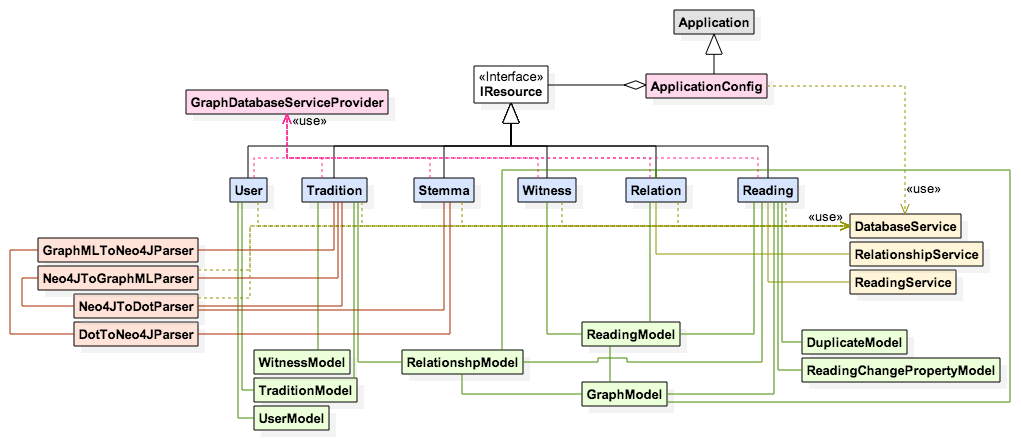
\includegraphics[scale=0.40]{ProjectOverview.png}
\end{figure}
This overview shows the relation between the classes of the StemmaREST service. As StemmaREST is based on the Jersey Framework all the provided Resources need to be registered in this framework. This is done in the ApplicationConfig class, like it is specified in the chapter Jersey. All classes which should be registered as a 'resource' need to implement the IResource Interface. \\
All IResources which need access to the Database use the GraphDatabaseServiceProvider. The GraphDatabaseServiceProvider contains a static GraphDatabaseServiceObject which can be requested by the IResource and used to acces the Database.\\
Several IResources need the service classes to share common functionality.\\
The model classes are dataclasses which contain the datamodels. They are also used for the serialisation and deserialisation of xml and JSON strings. For this serialisation the jackson package is used.\\
The parser classes are used to import graphml and dot files into the database.

\begin{figure}[h!]
  \caption{Request Sequence}
  \centering
    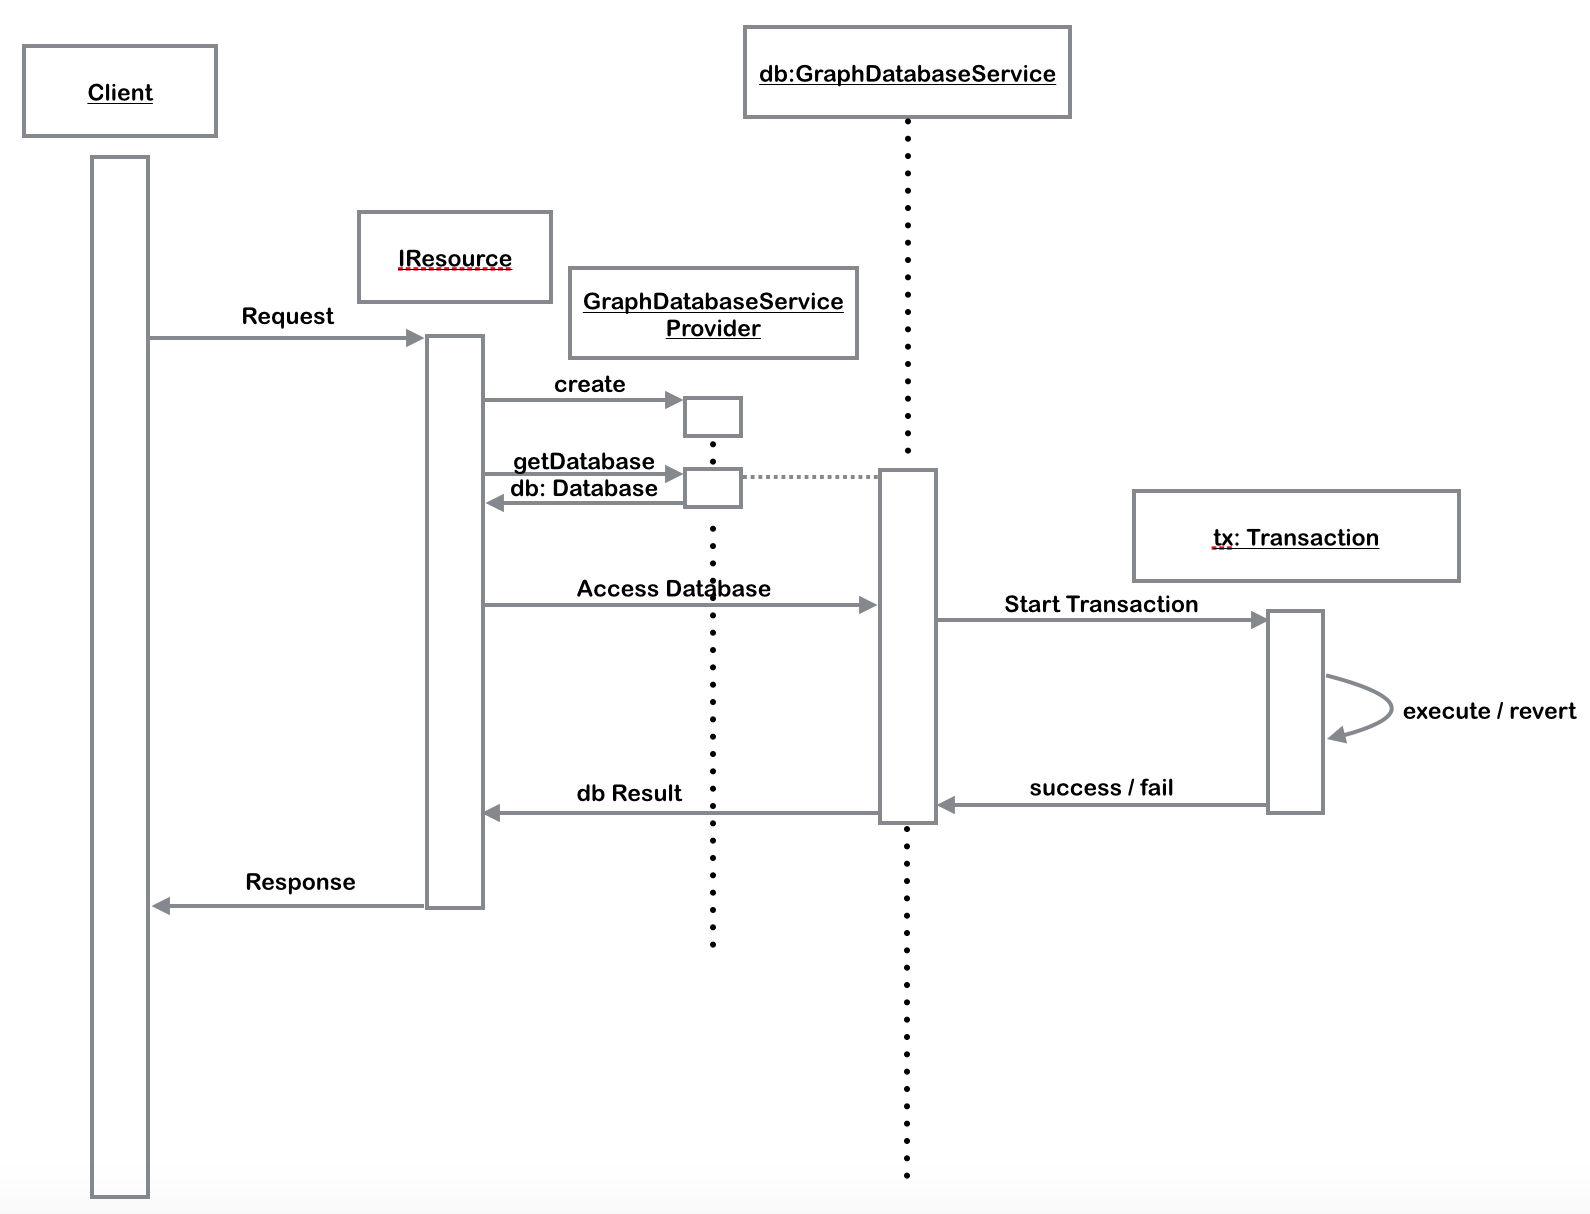
\includegraphics[scale=0.40]{stdRequest.png}
\end{figure}
When a client sends a request to the stemmaREST service. Jersey instantiates the requested IResource. GraphDatabaseServiceProvided is instantiated to request the singleton database. All requests require access to the database. The transaction is executed in the manner the request requires and a response is sent to the client. 
\\ \quad \\
More information about the database design and the Jersey integration can be found in the chapters Database and Jersey. 
\\ \quad \\
A more detailed Class-Overview can be found:
\url{https://github.com/tohotforice/PSE2_DH/blob/master/Dokumentation/DetailedClassOverview.svg}

%----------------------------------------------------------------------------------------
%	CHAPTER 2
%----------------------------------------------------------------------------------------

\chapterimage{header.png} % Chapter heading image

\chapter{Database (neo4j)}

In this project a graph database is used to store the data. This was done as graph databases are much faster when it comes down to look for objects in a list that contain some constraints to other objects. \\ In a relational database one would normally use multiple joins to get the desired result, but by using a graph this task becomes much easier since it is possible to traverse the graph from node to node using either breadth- or depth-first algorithms for a specific relation between nodes. This method makes a search for nodes, representing objects, which are connected to each other, very efficient. \\ \quad \\ Neo4J was chosen(more information can be found at http://neo4j.com/developer/graph-db-vs-rdbms/), which is a graph database capable of very efficiently managing nodes and relationship even in a large scale graph.\\
Additional information regarding performance could be found in the related chapter of this documentation. \\ \quad \\The stemmaweb database is basically a one big graph, with different labels marking different nodes and relationships. \\ \quad \\Those labels are used in the database:\\ \quad \\
\begin{tabular}{|l|l|}
\hline 
\textbf{Nodes} & \textbf{Relationships} \\ 
\hline 
ROOT & RELATIONSHIP \\ 
\hline 
STEMMA & STEMMA \\ 
\hline 
WITNESS & NORMAL \\ 
\hline 
TRADITION &  \\ 
\hline 
USER &  \\ 
\hline 
WORD &  \\ 
\hline 
\end{tabular} \\\\
Since each label is stored in another file, searching or traversing the graph is highly efficient. \\ \quad \\ The database structure is as follows:
\begin{center}
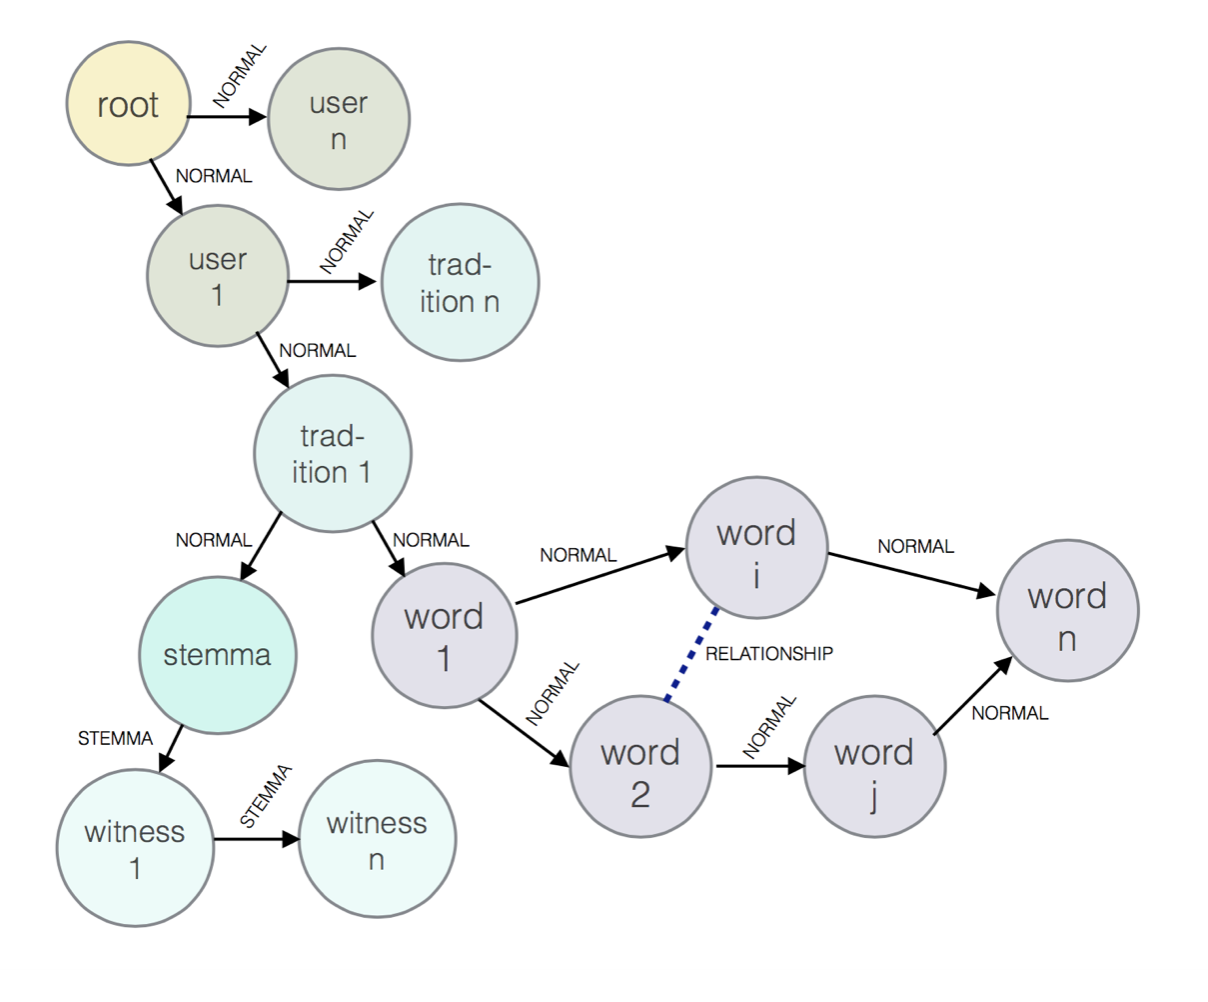
\includegraphics[scale=.5]{Pictures/database.png} 
\end{center} 
Neo4J uses a script language called cypher. Cypher is a declarative graph query language that allows for expressive and efficient querying and updating of the graph store. Cypher queries, though, need to be interpreted and translated into an execution plan. This is the reason why they are not always as fast as the native java traversal API, which has therefore become the common query tool used in the project.


%----------------------------------------------------------------------------------------
%	CHAPTER 3
%----------------------------------------------------------------------------------------

\chapterimage{header.png} % Chapter heading image

\chapter{Jersey}

\section*{Introduction}
Jersey is an open source java framework for developing RESTful Web Services in Java that is built upon JAX-RS and serves as a JAX-RS Reference Implementation. It adds additional features and utilities in order to further simplify development of REST-APIs. Jersey helps support exposing the data in different media types, including JSON, which is very frequently used in this project. 

\section*{Method Declarations}
An example of the method declaration of duplicateReading in the reading class:

\begin{lstlisting}
@POST
@Path("duplicatereading")
@Consumes(MediaType.APPLICATION_JSON)
@Produces(MediaType.APPLICATION_JSON)
public Response duplicateReading(DuplicateModel duplicateModel)
\end{lstlisting}

The @POST annotation states the http method.\\
The @Path annotation sets the url path.\\
The method "consumes" (i.e. gets from the client side) data sent by the client, in this case a java object of a "DuplicateModel" which is passed with the call as a JSON object and then gets parsed by the server into a POJO. The method "produces" (returns) a response, which is the method's return value, in this case also in JSON. 
\\\\
Another example from the witness class:

\begin{lstlisting}
@GET
@Path("gettext/fromtradition/{tradId}/ofwitness/{witnessId}")
@Produces(MediaType.APPLICATION_JSON)
public Response getWitnessAsText(@PathParam("tradId") String tradId,		
	@PathParam("witnessId") String witnessId) {
\end{lstlisting}

The values in curly braces in the path (tradId and witnessId) are path parameters, which are used in the method. In this example they are given in the URL and not as JSON. In the method declaration they are annotated with @PathParam. 

\section*{IResources}
In the ApplicationConfig class all the IResources (the objects) are loaded in the following method:

\begin{lstlisting}
@Override
public Set<Class<?>> getClasses() {
	Set<Class<?>> s = new HashSet<Class<?>>();
	s.add(Witness.class);
	s.add(User.class);
	s.add(Tradition.class);
	s.add(Relation.class);
	s.add(Stemma.class);
	s.add(Reading.class);
	
	return s;
}
\end{lstlisting}

An 'IResource' is a class that provides methods annotated with @GET, @POST, @PUT or @DELETE. All the API calls that can be made using stemmarest are defined in those six classes: Witness, User, Tradition, Relation, Stemma and Reading.
\\

\begin{lstlisting}
@Path("/reading")
public class Reading implements IResource {
\end{lstlisting}

%----------------------------------------------------------------------------------------
%	CHAPTER 4
%----------------------------------------------------------------------------------------

\chapterimage{header.png} % Chapter heading image

\chapter{Performance}

One of the main goals of this project was to create a RESTful service which is significantly faster then the existing one. To verify the speed of the service some performance tests are done. 
\\ \quad \\
The goal of the performance tests is to show that the response time of the service is limited and within a usable range. The performance (benchmark) tests therefore measure the time needed to execute all operations for a certain request. This includes the time to transmit the data over HTTP, the time to execute the internal algorithms and the time to access the database. All the Data is transmitted over the local loop interface. The network speed is therefore not measured. 
\\ \quad \\
For the purpose of the tests the database is being populated by a random graph which contains several valid traditions on which the REST requests can be executed. Several tests with databases of different sizes are done to show that the response time does not change as the size of the database increases.
\\ \quad \\
The first set of diagrams show the result of tests with different database sizes. Those tests show that the RESTful service response time is not influenced by the size of the database in a significant way. This is related to the use of the Graphdatabase in which a query can search a subgraph without filtering the whole database. 
\begin{remark}
The implementation of stemmarest uses some search-node-by-id methods (a part of Neo4j framework) which search over the complete database. It is important to realize that those quarries are done in $O(log n)$ time and are not seen in the noise of the other operations during the tests. This can be seen in the diagrams in such methods as \textit{getReading}, \textit{getNextReading} etc, which use the search-node-by-id method and their execution time hardly change even in a very big data base. In a much larger Database those methods will slow down the REST requests, though it is not expected that the database will grow so big that such operations will have any impact.
\end{remark} 

\begin{figure}[h!]
  \caption{Database with 1000 nodes,  working tradition with 100 nodes }
  \centering
    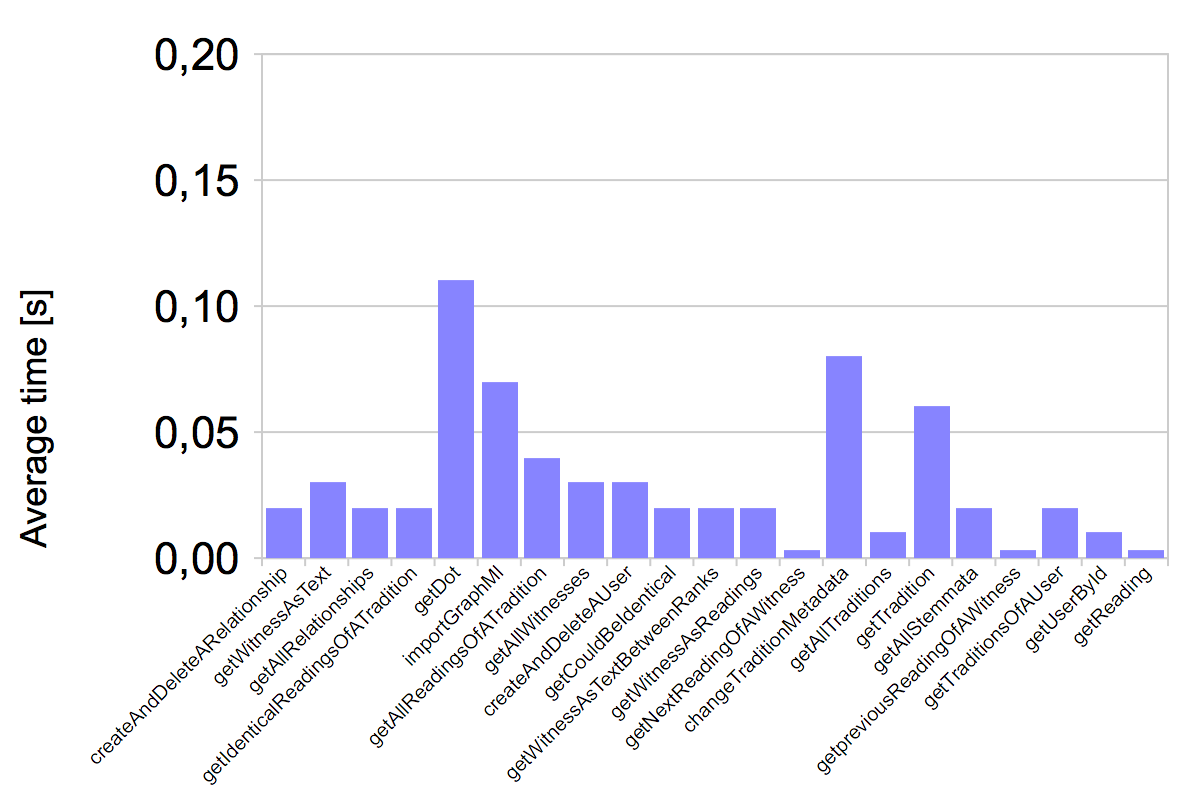
\includegraphics[scale=0.45]{1knode.png}
\end{figure}

\begin{figure}[h!]
  \caption{Database with 100000 nodes,  working tradition with 100 nodes }
  \centering
    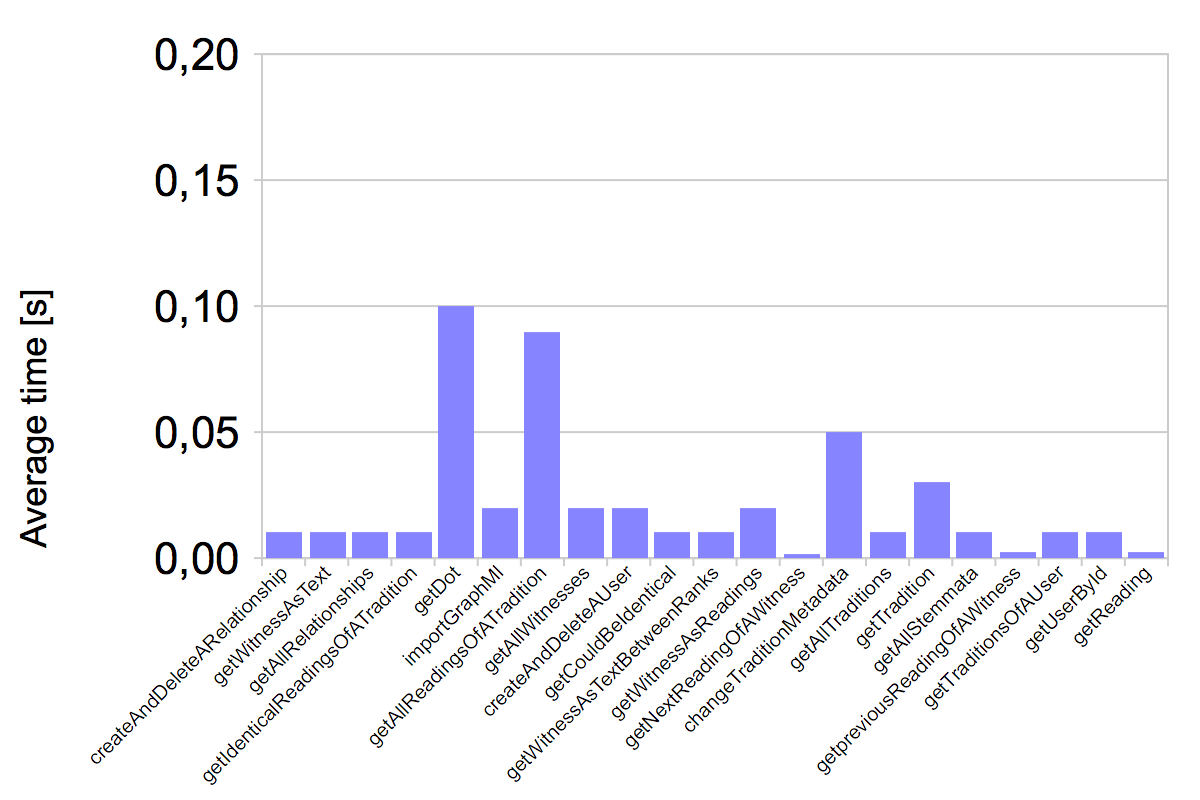
\includegraphics[scale=0.45]{100knode.png}
\end{figure}

\begin{figure}[h!]
  \caption{Database with 1000000 nodes,  working tradition with 100 nodes }
  \centering
    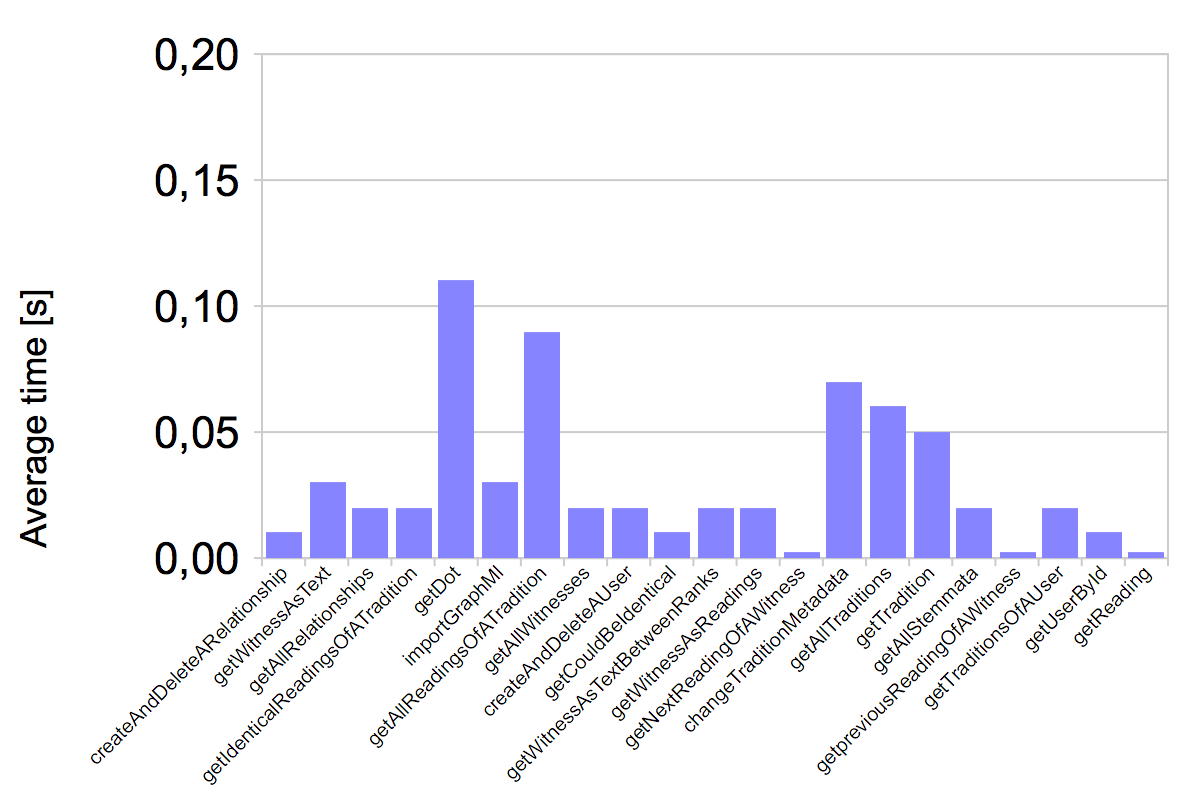
\includegraphics[scale=0.45]{1000knode.png}
\end{figure}
In those diagrams it is possible to see that the response time is almost independent to the database size between 1000 and 1 Million Nodes (Readings). As explained before, this is the result of the fact that each Tradition can be selected as a subgraph and the algorithms only have to search it, rather than the whole database. It is obvious, though, that the tradition size have an influence on the speed of the implemented algorithms as the working subset, which is in most cases a tradition, grows with a bigger tradition. Most of the algorithms which work on a tradition are in $O(log n)$, though there are also some export and import functions which have to handle each node and relation of the tradition and run in $O(n)$. 
\\ \quad \\
The following diagrams show the results of the tests in which the dimension of the tradition is varied while the size of the database stays the same. 
\begin{figure}[h!]
  \caption{Database with 10000 nodes,  working tradition with 1000 nodes }
  \centering
    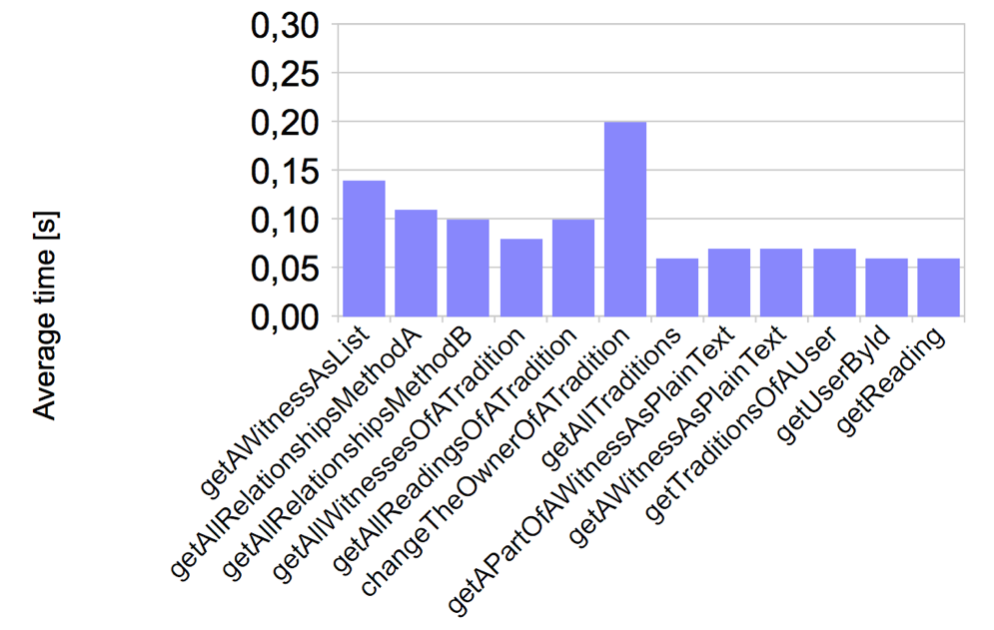
\includegraphics[scale=0.45]{trad1kwords.png}
\end{figure}
\begin{figure}[h!]
  \caption{Database with 10000 nodes,  working tradition with 10000 nodes }
  \centering
    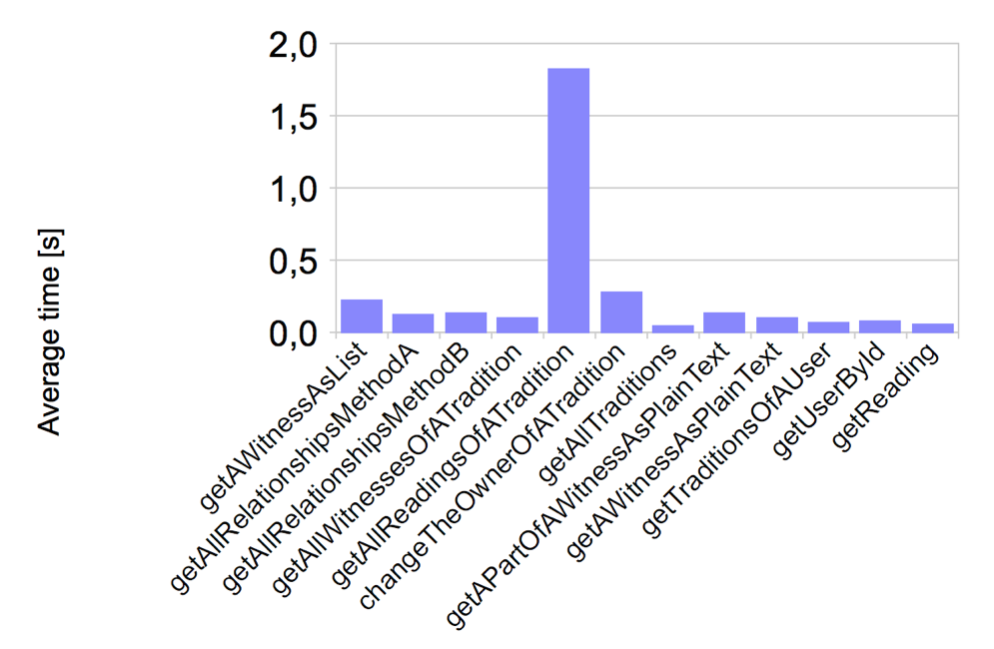
\includegraphics[scale=0.45]{trad10kwords.png}
\end{figure}
According to the diagrams, the execution time depends on the size of the working tradition, as can be seen in the results for the getAllReadingsFromATradition method, in which each reading of the tradition is parsed to a JSON Object and all are returned as an List. The parsing of those nodes executes in O(n) time and the downloading of the JSON file takes about the same. As larger traditions are not expected the execution time of those methods stays in the accepted range.

%----------------------------------------------------------------------------------------
%	PART
%----------------------------------------------------------------------------------------

\part{Testing}

%----------------------------------------------------------------------------------------
%	CHAPTER 5
%----------------------------------------------------------------------------------------

\chapterimage{header.png} % Chapter heading image

\chapter{Concept}
This chapter describes the test-concept of the Project. The tests were used for test driven development and to assure the quality of the product. All tests are written in such a manner that they do not have any impact on the architecture of the project.

\section*{Jersey Overview} 

\begin{center}
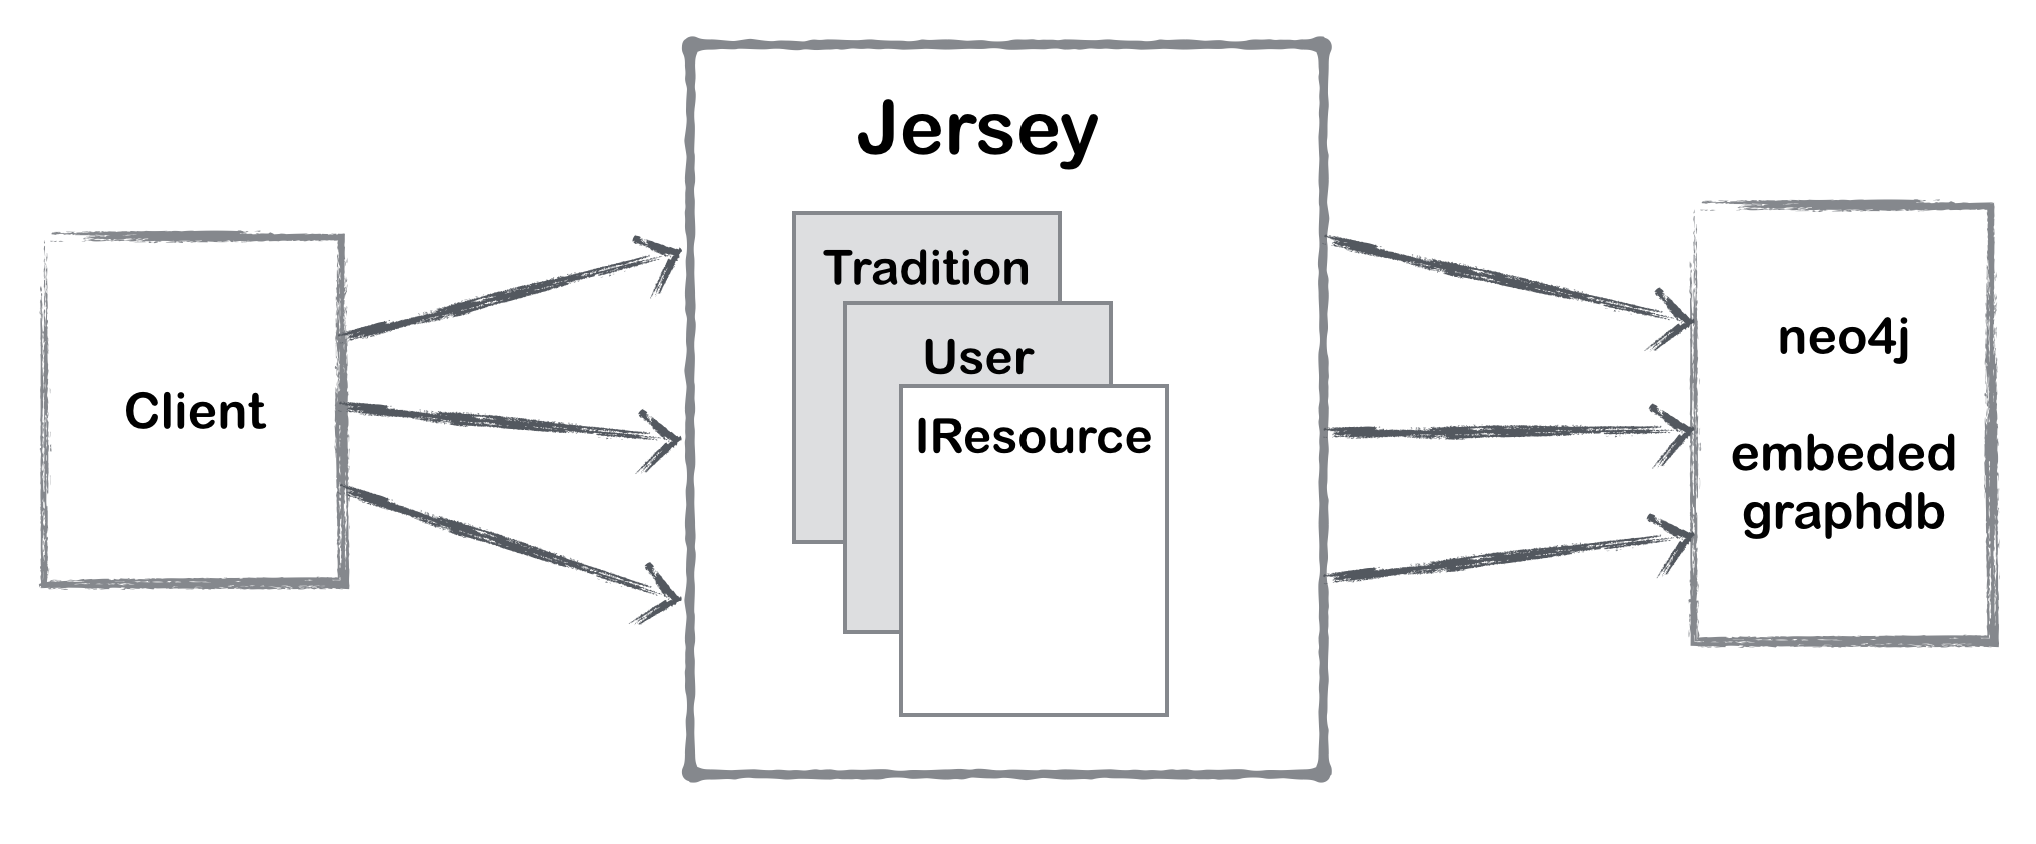
\includegraphics[scale=.40]{Pictures/jerseyoverview.png} 
\end{center}

For every REST call in the system a jersey instantiate the requested IResource and provides the service. A global singleton GraphDatabaseService object, which is is an embedded neo4j GraphDatabase, is used to provide the service. To achieve a minimal invasive test system the actual database is being replaced with a test database. To change the database with minimal test related code in the project, the GraphDatabaseServiceProvider is configured to return an impermanent Database. As the GraphDatabaseService is a singleton object this configuration is done before the start-up of the Jersey Testserver.

%----------------------------------------------------------------------------------------
%	CHAPTER 6
%----------------------------------------------------------------------------------------

\chapter{Configure the Test-Database}

To use an impermanent Testdatabase in the Tests the following initialization steps are done:
A Claswide GraphDatabaseService object db is registered:

\begin{lstlisting}[language=java]
    GraphDatabaseService db;
\end{lstlisting}
In the @Before method the singleton GraphDatabaseService provided by the GraphDatabaseServiceProvider is overwritten by the following line:

\begin{lstlisting}[language=java]
    GraphDatabaseServiceProvider.setImpermanentDatabase();
\end{lstlisting}
Later the db object is initialized by:
\begin{lstlisting}[language=java]
    db = new GraphDatabaseServiceProvider().getDatabase();
\end{lstlisting}
In the @After method the database is being closed:
\begin{lstlisting}[language=java]
    db.shutdown();
\end{lstlisting}

%----------------------------------------------------------------------------------------
%	CHAPTER 7
%----------------------------------------------------------------------------------------

\chapterimage{header.png} % Chapter heading image

\chapter{Integration Tests}

\begin{center}
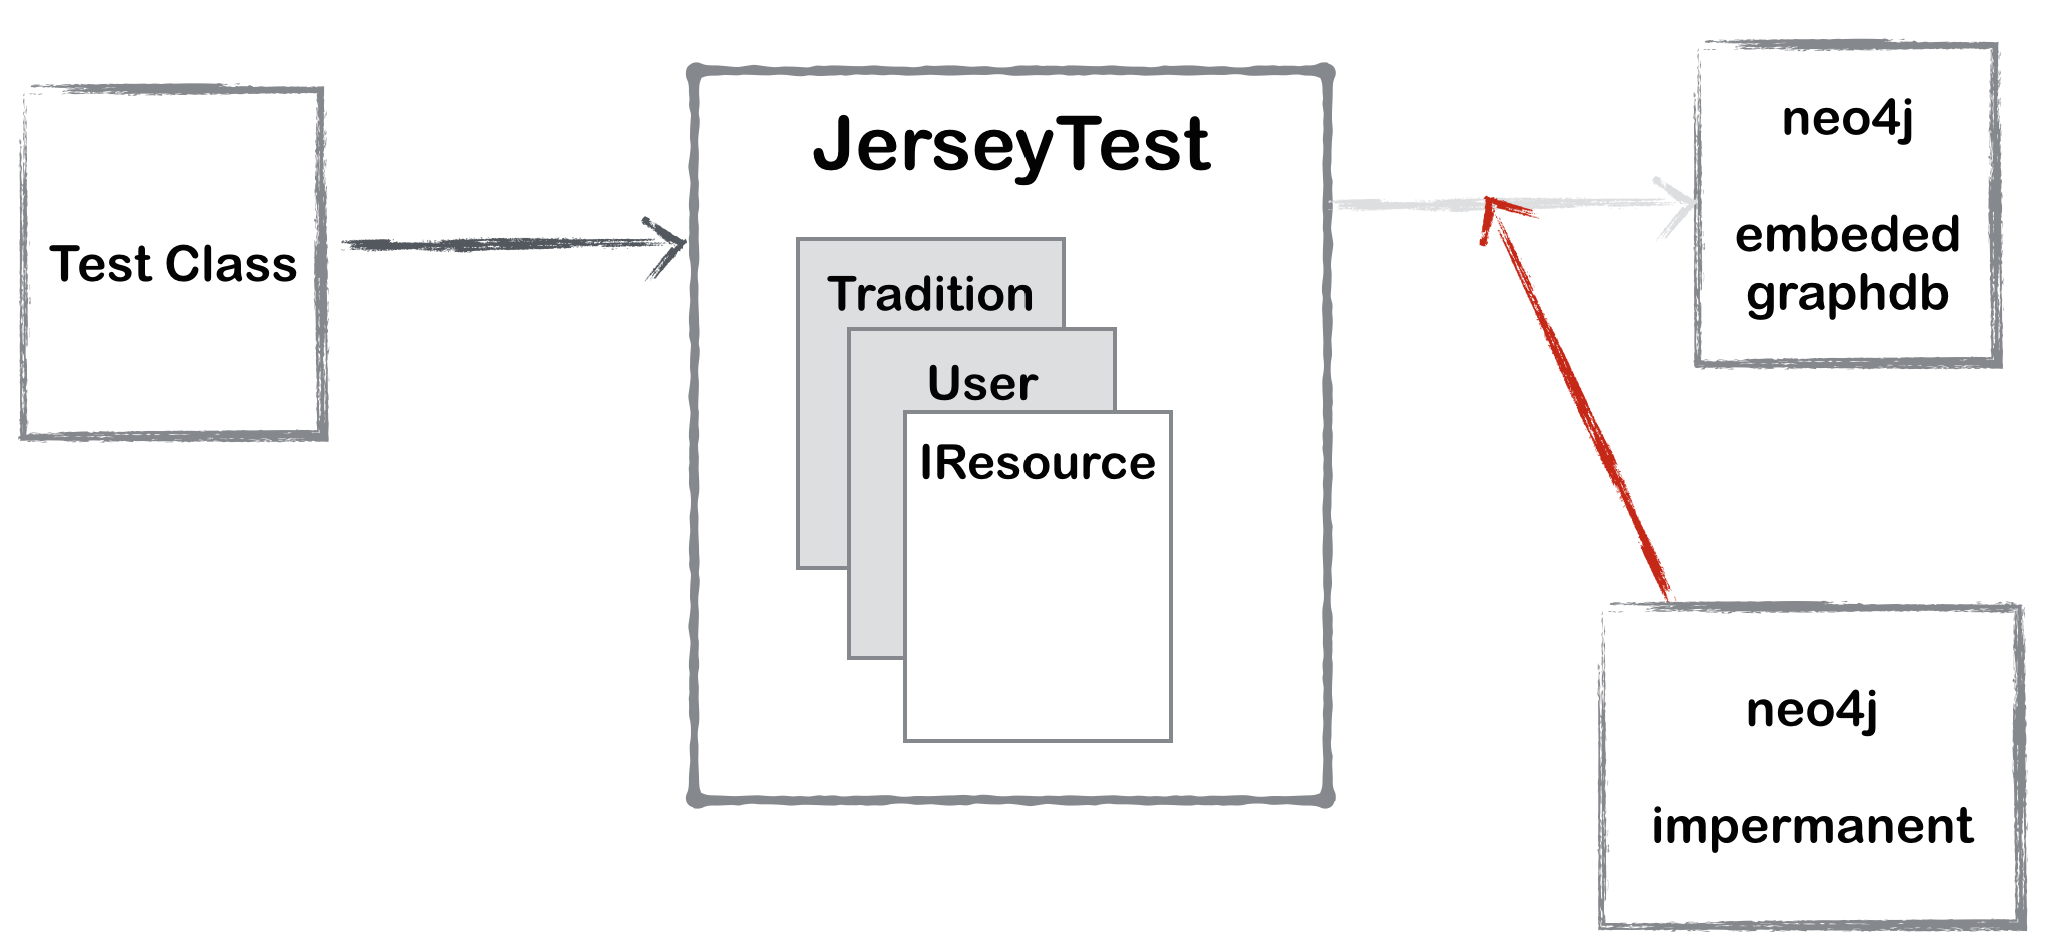
\includegraphics[scale=.4]{Pictures/jerseytestoverview.png} 
\end{center}

Every user story is tested with integration tests. Those tests are the mean of assuring the quality of the project. \\ \quad \\ To inject objects into a resource the resource must be created statically. This is not possible when the resources are instantiated only when a REST call occurs. To solve this problem JerseyTestServerFactory creates a server where instantiated resources can be registered.\\
To start a JerseyTestServer a global JerseyTest is created:
\begin{lstlisting}[language=java]
private JerseyTest jerseyTest;
\end{lstlisting}
The JerseyTestServerFactory creates a JerseyTest with already instantiated resources. This is used to inject the mock objects.\\
 Multiple resources can be added by chaining: .addResource(..).addResource()
\begin{lstlisting}[language=java]
jerseyTest = JerseyTestServerFactory.newJerseyTestServer()
	.addResource(userResource).create();
jerseyTest.setUp();
\end{lstlisting}

The test is done by calling a webresource of jerseyTest:
\begin{lstlisting}[language=java]
@Test
public void SimpleTest(){
  String actualResponse = jerseyTest.resource()
      .path("/user").get(String.class);
  assertEquals(actualResponse, "User!");
}
\end{lstlisting}

\subsection*{Example}
\url{https://github.com/tohotforice/PSE2_DH/blob/e364fcb0c164981281c5799a6bf9f9f9ea5eb503/stemmarest/src/test/java/net/stemmaweb/stemmaserver/UserTest.java}

%----------------------------------------------------------------------------------------
%	CHAPTER 8
%----------------------------------------------------------------------------------------

\chapterimage{header.png} % Chapter heading image

\chapter{Benchmark Testing}

The main goal of the stemmarest project was to achieve better performance then the previous service. To measure the performance of the system benchmark testing was needed. A benchmark test basically calls the RESTful service multiple times and measure the response time. To achieve this a JUnit benchmark test suite is used. The JUnitbenchmarks measures the time used to execute a test and can generate visual representations of the measurement.\\
For effective benchmark testing it is important to have a variety of different databases. Those databases should differ in size from small to very large.
To generate valid graphs only limited by space the class \textit{RandomGraphGenerator} is being used. By calling this static method a graph is generated according to the given parameters.\\
\begin{remark}
Please note that the response time depends highly on the hardware the tests are running on and the actual state of Javas virtual machine. 
\end{remark}
To reduce the influence of the virtual machine before the measurements 5 warm-up calls are done. The hardware which was used for testing is represented in the report.

\section*{Setup}
All the classes related to the Benchmark Tests can be found in the package \\ \textit{net.stemmaweb.stemmaserver.benachmarktests}. The class BenchmarkTests contains all the Tests. The classes Benchmark<n>Nodes contain the database generator. In it the number of nodes in the current test-database is being configured. BenchmarkTests cant be run as a JUnit test.

\begin{center}
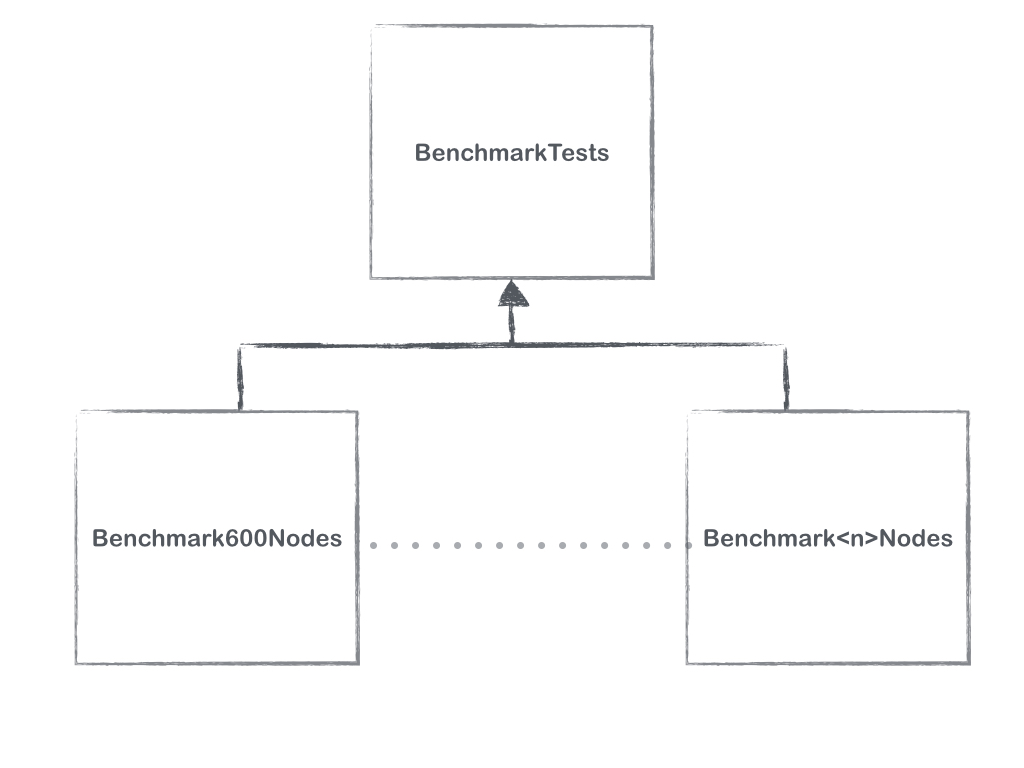
\includegraphics[scale=0.4]{BenchmarkTestsClassOverview.jpg} 
\end{center}

Tests are implemented in the BenchmarkTests class with the @Test annotation. Only restcall is implemented in the methods and they only test if the Response.Status is OK. This assures that as low as possible overhead time will be generated and measured.

\begin{remark}
JUnitBenchmarks measures the time to execute (@Before, @Test, @After). Heavy operations which should not be measured can be done in @BeforeClass and @AfterClass.
\end{remark}

To create a new database, the test-environment copies the class Benchmark600Nodes and rename it to the count of Nodes that are being inserted. In the class itself only two small adjustments are done: the name of the report file is being changed \textit{@BenchmarkMethodChart(filePrefix = ''benchmark/benchmark-600Nodes'')} and the properties of the database which should be generated are being adjusted \textit{rgg.role(db, 2, 1, 3, 100);}. role(databaseService, cardinalityOfUsers, cardinalityOfTraditionsPerUser, cardinalityOfWitnessesPerTradition, degreeOfTheTraditionGraphs)

\section*{Run Benchmarktests}
The Benchmarktests can be run as every JUnit test. To generate the report, though, an argument needs to be passed. 
Create a JUnit Test as follows:

\begin{center}
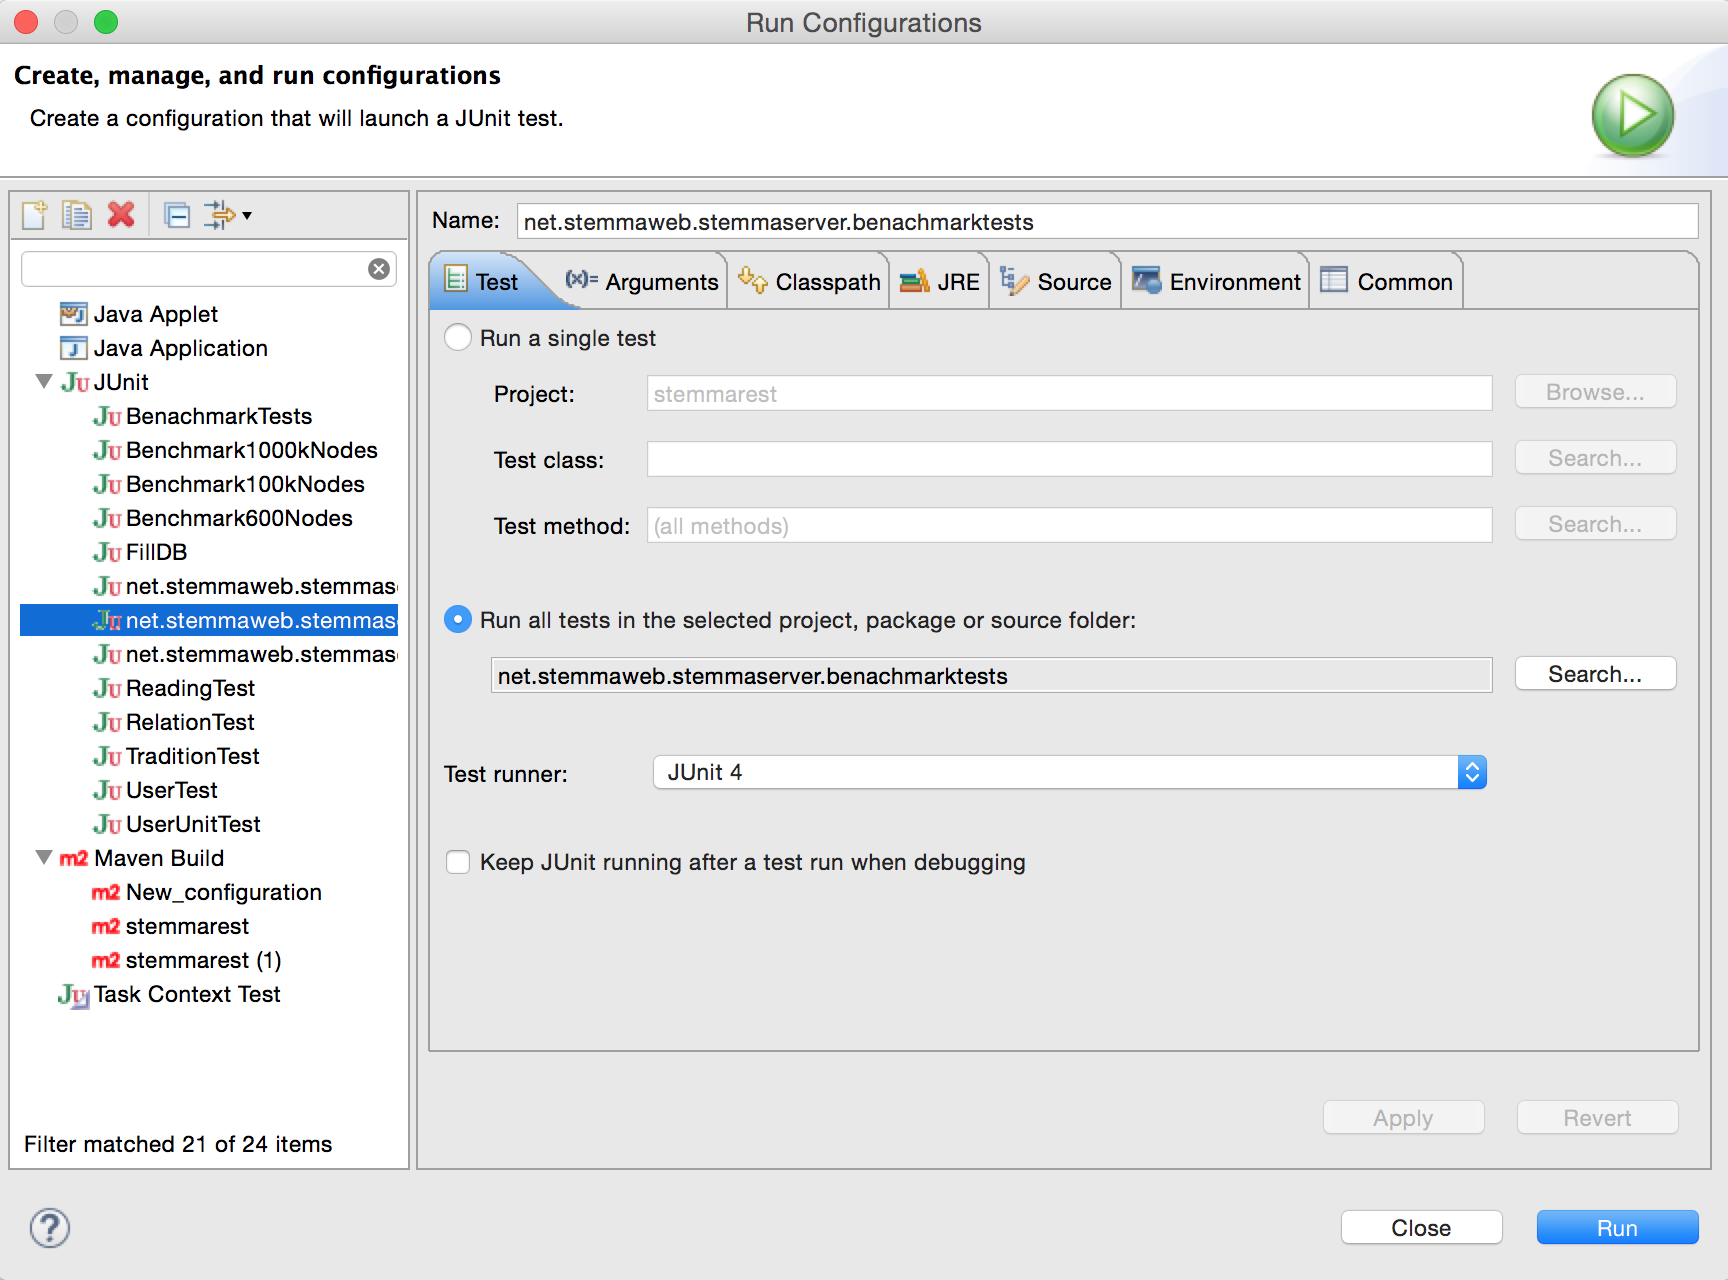
\includegraphics[scale=0.4]{benchmarkTest.png} 
\end{center}

\begin{center}
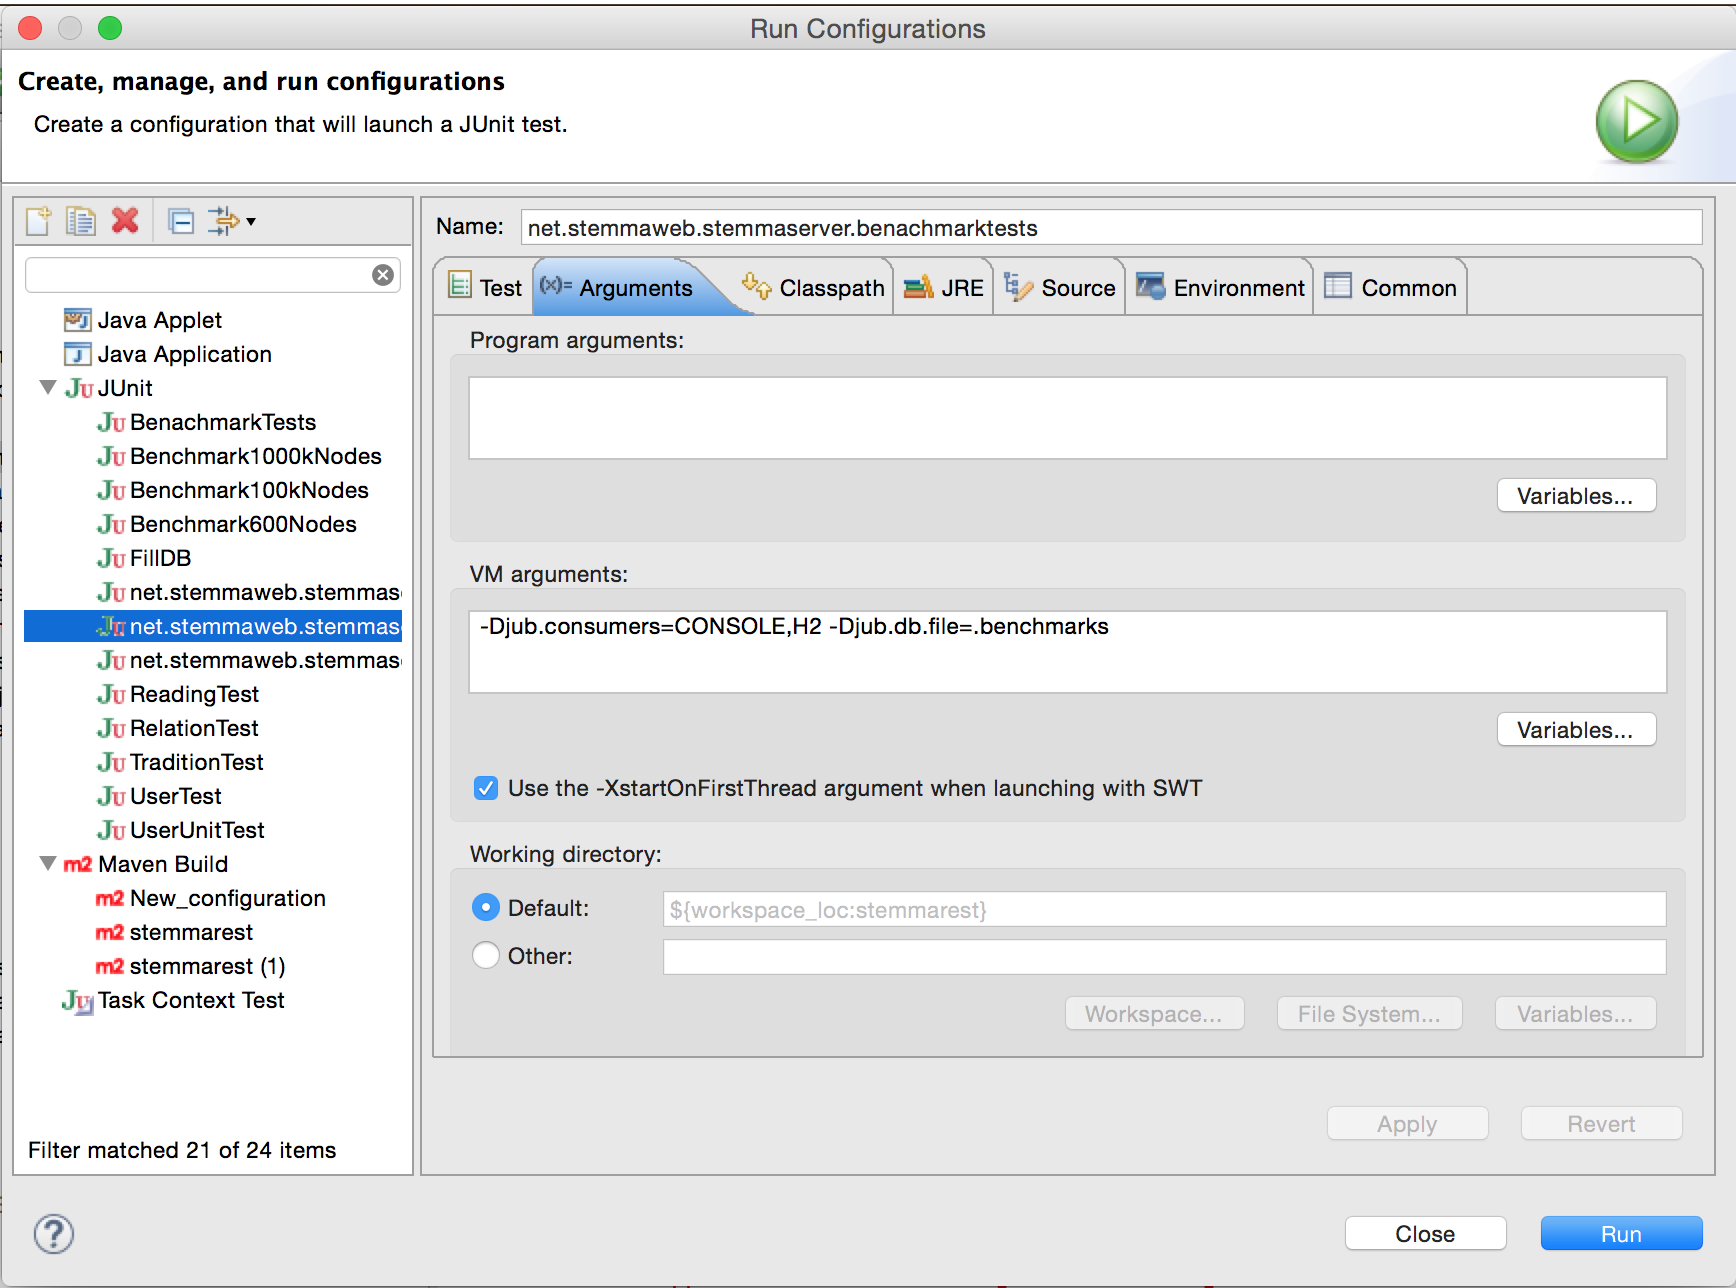
\includegraphics[scale=0.4]{benchmarkTestArgument.png} 
\end{center}

On the tab Arguments \textit{-Djub.consumers=CONSOLE,H2 -Djub.db.file=.benchmarks} has to be inserted into the VM Arguments input. After that the test can be executed as usual. After the execution of the tests the reports will be stored at \textit{benchmark/}.
 
\begin{remark}
The execution of the tests will take some time because of the need to generate huge graphs. Its recommended not to use the computer for other assignments during the tests.  
\end{remark}


%----------------------------------------------------------------------------------------
%	PART
%----------------------------------------------------------------------------------------

\part{RESTful API}

%----------------------------------------------------------------------------------------
%	CHAPTER 10
%----------------------------------------------------------------------------------------

\chapter{Services}
\section{Baseresource: }
http://localhost:8080/
\section{/stemma}
\textbf{Method Name: }getAllStemmata \\ Gets a list of all Stemmata available, as dot format
\begin{get}
/getallstemmata/fromtradition/\{tradId\}
\end{get}
\begin{response}
list of stemmata as dot
\end{response}
\begin{parameter}
tradId as string
\end{parameter}
\textbf{Method Name: }setStemma \\ Puts the Stemma of a DOT file in the database
\begin{post}
/newstemma/intradition/\{tradId\}
\end{post}
\begin{response}
stemma as dot
\end{response}
\begin{parameter}
tradId as string
\end{parameter}
\textbf{Method Name: }reorientStemma \\ Reorients a stemma tree with a given new root node
\begin{post}
/reorientstemma/fromtradition/\{tradId\}/withtitle/\{stemmaTitle\}/withnewrootnode/\{nodeId\}
\end{post}
\begin{response}
stemma as dot
\end{response}
\begin{parameter}
tradId as string
\end{parameter}
\begin{parameter}
stemmaTitle as string
\end{parameter}
\begin{parameter}
nodeId as string
\end{parameter}
\textbf{Method Name: }getStemma \\ Returns JSON string with a Stemma of a tradition in DOT format
\begin{get}
/getstemma/fromtradition/\{tradId\}/withtitle/\{stemmaTitle\}
\end{get}
\begin{response}
stemma as dot
\end{response}
\begin{parameter}
tradId as string
\end{parameter}
\begin{parameter}
stemmaTitle as string
\end{parameter}
\section{/relation}
\textbf{Method Name: }delete \\ Remove all relationships, as it is done in https://github.com/tla/stemmaweb/blob/master/lib/stemmaweb/Controller/Relation.pm line 271) in Relationships of type RELATIONSHIP between the two nodes.
\begin{post}
/deleterelationship/fromtradition/\{tradId\}
\end{post}
\begin{request}
relationshipModel as application/json
\end{request}
\begin{response}
 as text/plain: HTTP Response 404 when no node was found, 200 When relationships where removed
\end{response}
\begin{parameter}
tradId as string
\end{parameter}
\textbf{Method Name: }create \\ Creates a new relationship between the two nodes specified.
\begin{post}
/createrelationship
\end{post}
\begin{request}
relationshipModel as application/json
\end{request}
\begin{response}
graphModel as application/json
\end{response}
\textbf{Method Name: }getAllRelationships \\ Get a list of all relationships from a given tradition.
\begin{get}
/getallrelationships/fromtradition/\{tradId\}
\end{get}
\begin{response}
list of relationshipModel as application/json
\end{response}
\begin{parameter}
tradId as string
\end{parameter}
\textbf{Method Name: }deleteById \\ Removes a relationship by ID.
\begin{delete}
/deleterelationshipbyid/withrelationship/\{relationshipId\}
\end{delete}
\begin{response}
relationshipModel as application/json
\end{response}
\begin{parameter}
relationshipId as string
\end{parameter}
\section{/tradition}
\textbf{Method Name: }getAllRelationships \\ Gets a list of all relationships of a tradition with the given id.
\begin{get}
/getallrelationships/fromtradition/\{tradId\}
\end{get}
\begin{response}
list of relationshipModels as application/json
\end{response}
\begin{parameter}
tradId as string
\end{parameter}
\textbf{Method Name: }changeTraditionMetadata \\ Changes the metadata of the tradition.
\begin{post}
/changemetadata/fromtradition/\{tradId\}
\end{post}
\begin{request}
traditionModel as application/json
\end{request}
\begin{response}
traditionModel as application/json
\end{response}
\begin{parameter}
tradId as string
\end{parameter}
\textbf{Method Name: }getAllTraditions \\ Gets a list of all the complete traditions in the database.
\begin{get}
/getalltraditions
\end{get}
\begin{response}
list of traditionModels as application/json
\end{response}
\textbf{Method Name: }getAllWitnesses \\ Gets a list of all the witnesses of a tradition with the given id.
\begin{get}
/getallwitnesses/fromtradition/\{tradId\}
\end{get}
\begin{response}
list of witnessModels as application/json
\end{response}
\begin{parameter}
tradId as string
\end{parameter}
\textbf{Method Name: }getTradition \\ Returns GraphML file from specified tradition owned by user
\begin{get}
/gettradition/withid/\{tradId\}
\end{get}
\begin{response}
tradition as application/xml (graphML)
\end{response}
\begin{parameter}
tradId as string
\end{parameter}
\textbf{Method Name: }deleteTraditionById \\ Removes a complete tradition
\begin{delete}
/deletetradition/withid/\{tradId\}
\end{delete}
\begin{response}
 as text/plain: http response
\end{response}
\begin{parameter}
tradId as string
\end{parameter}
\textbf{Method Name: }importGraphMl \\ Imports a tradition by given GraphML file and meta data
\begin{post}
//newtraditionwithgraphml
\end{post}
\begin{request}
 graphML as multipart/form-data
\end{request}
\begin{response}
the id of the imported tradition as text/plain
\end{response}
\textbf{Method Name: }getDot \\ Returns DOT file from specified tradition owned by user
\begin{get}
/getdot/fromtradition/\{tradId\}
\end{get}
\begin{response}
 as application/json: XML data
\end{response}
\begin{parameter}
tradId as string
\end{parameter}
\section{/reading}
\textbf{Method Name: }changeReadingProperties \\ Changes properties of a reading according to its keys
\begin{post}
/changeproperties/ofreading/\{readId\}
\end{post}
\begin{request}
 ReadingChangePropertyModel as application/json
\end{request}
\begin{response}
readingModel as application/json
\end{response}
\begin{parameter}
readId as long
\end{parameter}
\textbf{Method Name: }getReading \\ Returns a single reading by global neo4j id
\begin{get}
/getreading/withreadingid/\{readId\}
\end{get}
\begin{response}
readingModel as application/json
\end{response}
\begin{parameter}
readId as long
\end{parameter}
\textbf{Method Name: }duplicateReading \\ Duplicates a reading in a specific tradition. Opposite of merge
\begin{post}
/duplicatereading
\end{post}
\begin{request}
duplicateModel as application/json
\end{request}
\begin{response}
GraphModel as application/json
\end{response}
\textbf{Method Name: }mergeReadings \\ Merges two readings into one single reading in a specific tradition. Opposite of duplicate
\begin{post}
/mergereadings/first/\{firstReadId\}/second/\{secondReadId\}
\end{post}
\begin{response}
 as application/json: Status.OK on success or Status.INTERNAL\_SERVER\_ERROR with a detailed message.
\end{response}
\begin{parameter}
secondReadId as long
\end{parameter}
\begin{parameter}
firstReadId as long
\end{parameter}
\textbf{Method Name: }splitReading \\ Splits up a single reading into several ones in a specific tradition. Opposite of compress
\begin{post}
/splitreading/ofreading/\{readId\}/withsplitindex/\{splitIndex\}
\end{post}
\begin{request}
 as text/plain
\end{request}
\begin{response}
GraphModel as application/json
\end{response}
\begin{parameter}
readId as long
\end{parameter}
\begin{parameter}
splitIndex as int
\end{parameter}
\textbf{Method Name: }getNextReadingInWitness \\ gets the next readings from a given readings in the same witness
\begin{get}
/getnextreading/fromwitness/\{witnessId\}/ofreading/\{readId\}
\end{get}
\begin{response}
readingModel as application/json
\end{response}
\begin{parameter}
readId as long
\end{parameter}
\begin{parameter}
witnessId as string
\end{parameter}
\textbf{Method Name: }getPreviousReadingInWitness \\ gets the previous readings from a given readings in the same witness
\begin{get}
/getpreviousreading/fromwitness/\{witnessId\}/ofreading/\{readId\}
\end{get}
\begin{response}
readingModel as application/json
\end{response}
\begin{parameter}
readId as long
\end{parameter}
\begin{parameter}
witnessId as string
\end{parameter}
\textbf{Method Name: }getAllReadings \\ Returns a list of all readings in a tradition
\begin{get}
/getallreadings/fromtradition/\{tradId\}
\end{get}
\begin{response}
list of readingModels as application/json
\end{response}
\begin{parameter}
tradId as string
\end{parameter}
\textbf{Method Name: }getIdenticalReadings \\ Get all readings which have the same text and the same rank between given ranks
\begin{get}
/getidenticalreadings/fromtradition/\{tradId\}/fromstartrank/\{startRank\}/toendrank/\{endRank\}
\end{get}
\begin{response}
list of list of readingModels as application/json
\end{response}
\begin{parameter}
endRank as long
\end{parameter}
\begin{parameter}
tradId as string
\end{parameter}
\begin{parameter}
startRank as long
\end{parameter}
\textbf{Method Name: }getCouldBeIdenticalReadings \\ Returns a list of a list of readingModels with could be one the same rank without problems
\begin{get}
/couldbeidenticalreadings/fromtradition/\{tradId\}/fromstartrank/\{startRank\}/toendrank/\{endRank\}
\end{get}
\begin{response}
list of readingModels as application/json
\end{response}
\begin{parameter}
endRank as long
\end{parameter}
\begin{parameter}
tradId as string
\end{parameter}
\begin{parameter}
startRank as long
\end{parameter}
\textbf{Method Name: }compressReadings \\ Compress two readings into one. Texts will be concatenated together (with or without a space or extra text. The reading with the lower rank will be given first. Opposite of split
\begin{post}
/compressreadings/read1id/\{read1Id\}/read2id/\{read2Id\}/concatenate/\{con\}
\end{post}
\begin{request}
 as text/plain
\end{request}
\begin{response}
 as application/json: status.ok if compress was successful. Status.INTERNAL\_SERVER\_ERROR with a detailed message if not concatenated
\end{response}
\begin{parameter}
read1Id as long
\end{parameter}
\begin{parameter}
read2Id as long
\end{parameter}
\begin{parameter}
con as string
\end{parameter}
\section{/witness}
\textbf{Method Name: }getWitnessAsText \\ finds a witness in the database and returns it as a string
\begin{get}
/gettext/fromtradition/\{tradId\}/ofwitness/\{witnessId\}
\end{get}
\begin{response}
witness as string
\end{response}
\begin{parameter}
tradId as string
\end{parameter}
\begin{parameter}
witnessId as string
\end{parameter}
\textbf{Method Name: }getWitnessAsTextBetweenRanks \\ find a requested witness in the data base and return it as a string according to define start and end readings (including the readings in those ranks). if end-rank is too high or start-rank too low will return till the end/from the start of the witness
\begin{get}
/gettext/fromtradition/\{tradId\}/ofwitness/\{witnessId\}/fromstartrank/\{startRank\}/toendrank/\{endRank\}
\end{get}
\begin{response}
witness as string
\end{response}
\begin{parameter}
endRank as string
\end{parameter}
\begin{parameter}
tradId as string
\end{parameter}
\begin{parameter}
startRank as string
\end{parameter}
\begin{parameter}
witnessId as string
\end{parameter}
\textbf{Method Name: }getWitnessAsReadings \\ finds a witness in the database and returns it as a list of readings
\begin{get}
/getreadinglist/fromtradition/\{tradId\}/ofwitness/\{witnessId\}
\end{get}
\begin{response}
list of readingModels as application/json
\end{response}
\begin{parameter}
tradId as string
\end{parameter}
\begin{parameter}
witnessId as string
\end{parameter}
\section{/user}
\textbf{Method Name: }create \\ Creates a user based on the parameters submitted in JSON.
\begin{post}
/createuser
\end{post}
\begin{request}
userModel as application/json
\end{request}
\begin{response}
userModel as application/json
\end{response}
\textbf{Method Name: }getUserById \\ Gets a user by the id.
\begin{get}
/getuser/withid/\{userId\}
\end{get}
\begin{response}
userModel as application/json
\end{response}
\begin{parameter}
userId as string
\end{parameter}
\textbf{Method Name: }deleteUserById \\ Removes a user and all his traditions
\begin{delete}
/deleteuser/withid/\{userId\}
\end{delete}
\begin{response}
 as text/plain: OK on success or an ERROR in JSON format
\end{response}
\begin{parameter}
userId as string
\end{parameter}
\textbf{Method Name: }getTraditionsByUserId \\ Get all Traditions of a user
\begin{get}
/gettraditions/ofuser/\{userId\}
\end{get}
\begin{response}
 as application/json: OK on success or an ERROR in JSON format
\end{response}
\begin{parameter}
userId as string
\end{parameter}


%----------------------------------------------------------------------------------------
%	CHAPTER 11
%----------------------------------------------------------------------------------------

\chapter{Models}

\section{relationshipModel}
\begin{property}
a\_derivable\_from\_b as string
\end{property}
\begin{property}
alters\_meaning as string
\end{property}
\begin{property}
annotation as string
\end{property}
\begin{property}
b\_derivable\_from\_a as string
\end{property}
\begin{property}
displayform as string
\end{property}
\begin{property}
extra as string
\end{property}
\begin{property}
id as string
\end{property}
\begin{property}
is\_significant as string
\end{property}
\begin{property}
non\_independent as string
\end{property}
\begin{property}
reading\_a as string
\end{property}
\begin{property}
reading\_b as string
\end{property}
\begin{property}
scope as string
\end{property}
\begin{property}
source as string
\end{property}
\begin{property}
target as string
\end{property}
\begin{property}
type as string
\end{property}
\begin{property}
witness as string
\end{property}
\section{readingModel}
\begin{property}
grammar\_invalid as string
\end{property}
\begin{property}
id as string
\end{property}
\begin{property}
is\_common as string
\end{property}
\begin{property}
is\_end as string
\end{property}
\begin{property}
is\_lacuna as string
\end{property}
\begin{property}
is\_lemma as string
\end{property}
\begin{property}
is\_nonsense as string
\end{property}
\begin{property}
is\_ph as string
\end{property}
\begin{property}
is\_start as string
\end{property}
\begin{property}
join\_next as string
\end{property}
\begin{property}
join\_prior as string
\end{property}
\begin{property}
language as string
\end{property}
\begin{property}
lexemes as string
\end{property}
\begin{property}
normal\_form as string
\end{property}
\begin{property}
rank as long
\end{property}
\begin{property}
text as string
\end{property}
\section{traditionModel}
\begin{property}
id as string
\end{property}
\begin{property}
isPublic as string
\end{property}
\begin{property}
language as string
\end{property}
\begin{property}
name as string
\end{property}
\begin{property}
ownerId as string
\end{property}
\section{duplicateModel}
\begin{property}
readings as long
\end{property}
\begin{property}
witnesses as string
\end{property}
\section{graphModel}
\begin{property}
readings as long
\end{property}
\begin{property}
witnesses as string
\end{property}
\section{witnessModel}
\begin{property}
id as string
\end{property}
\section{userModel}
\begin{property}
id as string
\end{property}
\begin{property}
isAdmin as string
\end{property}
\section{ReadingChangePropertyModel}
\begin{property}
properties as list of KeyPropertyModels
\end{property}
\section{stemma}
A tree that provides an overview over the witnesses of a tradition. The relations between the witnesses which are displayed as nodes is central. Here the stemmata are mostly returned in dot format.
\section{GraphML}
\url{http://de.wikipedia.org/wiki/GraphML}
\section{KeyPropertyModel}
\begin{property}
key as string
\end{property}
\begin{property}
property as string
\end{property}

%----------------------------------------------------------------------------------------
%	BIBLIOGRAPHY
%----------------------------------------------------------------------------------------

%\chapter*{Bibliography}
%\addcontentsline{toc}{chapter}{\textcolor{ocre}{Bibliography}}
%\section*{Books}
%\addcontentsline{toc}{section}{Books}
%\printbibliography[heading=bibempty,type=book]
%\section*{Articles}
%\addcontentsline{toc}{section}{Articles}
%\printbibliography[heading=bibempty,type=article]

%----------------------------------------------------------------------------------------
%	INDEX
%----------------------------------------------------------------------------------------

%\cleardoublepage
%\phantomsection
%\setlength{\columnsep}{0.75cm}
%\addcontentsline{toc}{chapter}{\textcolor{ocre}{Index}}
%\printindex

%----------------------------------------------------------------------------------------

\end{document}